\section{Lực từ - Cảm ứng từ}
\subsection{Tóm tắt lí thuyết}
\begin{tomtat}
	\subsubsection{Độ lớn cảm ứng từ}
	\begin{dn}
		Cảm ứng từ $\vec{B}$ là một đại lượng vector, đặc trưng cho từ trường về phương diện tác dụng lực. Cảm ứng từ tại một điểm trong từ trường có:
		\begin{itemize}
			\item Phương trùng với phương của nam châm thử nằm cân bằng tại điểm đó.
			\item Chiều từ cực  Nam sang cực Bắc của nam châm thử.
			\item Độ lớn được xác định bằng biểu thức:
			\begin{equation}
				B=\dfrac{F}{IL\sin\theta}
			\end{equation}
		\end{itemize}
	\end{dn}
	Trong hệ SI, cảm ứng từ có đơn vị là tesla $\left(\si{\tesla}\right)$. Đơn vị tesla là đơn vị dẫn xuất, có mối liên hệ với các đơn vị cơ bản theo biểu thức:
	\begin{equation}
		\SI{1}{\tesla}=\SI{1}{\dfrac{\newton}{\ampere\cdot\meter}}
	\end{equation}
	$\SI{1}{\tesla}$ là độ lớn của cảm ứng từ của một từ trường đều mà khi đặt một dây dẫn có chiều dài $\SI{1}{\meter}$ mang dòng điện có cường độ $\SI{1}{\ampere}$ vào trong từ trường đó và vuông góc với vector cảm ứng từ thì dây dẫn sẽ chịu một lực từ có độ lớn $\SI{1}{\newton}$.
	\subsubsection{Lực từ tác dụng lên đoạn dây dẫn mang dòng điện}
	\paragraph{Độ lớn lực từ}
	\begin{boxdl}
			Lực từ tác dụng lên một đoạn dây dẫn mang dòng điện đặt trong từ trường đều được tính bởi biểu thức:
		\begin{equation}
			F=ILB\sin\theta
		\end{equation}
	\end{boxdl}

	\begin{center}
		\begin{tikzpicture}
			\coordinate (O) at(0,0);
			\coordinate (A) at($(O)+(30:3)$);
			\coordinate (B) at($(O)+(-60:3)$);
			\coordinate (C) at(2.5,0);
			\tkzMarkRightAngle[size=0.7,color=blue, line width=1.5pt](B,O,C);
			\node [cylinder, fill=gray!30!white, line width=1pt, shape border rotate=180, draw, minimum height=8.0cm, minimum width=0.6cm] at (O) {};
			\draw[-stealth,line width=2pt, red] (-2,0)--(3,0);
			\tkzMarkRightAngle[size=0.4,color=blue, line width=1.5pt](B,O,A);
			\draw[-stealth, line width=2pt] (O)--(A);
			\draw[-stealth, line width=2pt] (O)--(B);
			\fill   (O) circle[radius=3pt];
			\node[above] at (A) {$\vec{B}$};
			\node[below] at ($(C)-(0,0.3)$) {$\vec{IL}$};
			\node[right] at (B) {$\vec{F}$};
			\tkzMarkAngle[size=0.75cm,color=purple, line width=1.5pt](C,O,A);
			\tkzLabelAngle[color=black,pos=1.2](C,O,A){$\theta$};
		\end{tikzpicture}
	\end{center}
	trong đó:
	\begin{itemize}
		\item $F$: độ lớn lực từ tác dụng lên đoạn dây, đơn vị trong hệ SI là $\left(\si{\meter}\right)$;
		\item $B$: độ lớn cảm ứng từ, đơn vị trong hệ SI là $\left(\si{\tesla}\right)$;
		\item $I$: cường độ dòng điện qua đoạn dây, đơn vị trong hệ SI là $\left(\si{\ampere}\right)$;
		\item $L$: chiều dài đoạn dây, đơn vị trong hệ SI là $\left(\si{\meter}\right)$;
		\item $\theta$: góc hợp bởi vector $\vec{B}$ và vector phần tử dòng điện $\vec{IL}$.
	\end{itemize}
	\paragraph{Phương và chiều của lực từ}
	Lực từ tác dụng lên đoạn dây dẫn mang dòng điện trong từ trường đều có:
	\begin{itemize}
		\item Điểm đặt là tại trung điểm của đoạn dây.
		\item Phương vuông góc với mặt phẳng chứa đoạn dây dẫn mang dòng điện và vector cảm ứng từ.
		\item Chiều được xác định bằng quy tắc bàn tay trái:\\
		Đặt bàn tay trái sao cho các đường sức từ hướng vào lòng bàn tay, chiều từ cổ tay đến các ngón tay trùng với chiều dòng điện, khi đó ngón cái choãi ra $\SI{90}{\degree}$ chỉ chiều của lực từ tác dụng lên dòng điện.
		\begin{center}
			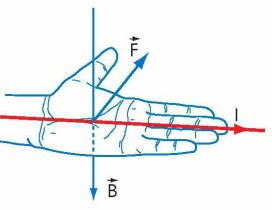
\includegraphics[width=0.3\linewidth]{figs/VN12-Y24-PH-SYL-017-8}
			\captionof{figure}{Hình vẽ mô tả quy tắc bàn tay trái.}
		\end{center}
	\end{itemize}
\end{tomtat}


\subsection{Ví dụ minh hoạ}
\begin{dang}{Vận dụng quy tắc bàn tay trái để xác định lực từ tác dụng đoạn dây dẫn mang dòng điện}
	\end{dang}
\begin{vd}
	Với mỗi trường hợp như hình, hãy xác định xem có lực từ tác dụng lên mỗi dây dẫn mang dòng điện hay không? Nếu có, hãy cho biết hướng của chúng.
	\begin{center}
		\begin{longtable}{M{8cm}M{8cm}}
			\begin{tikzpicture}
				\foreach \i in {0,1,...,4}
				\draw[blue, line width=1pt, decoration={markings, mark=at position 0.75 with {\arrow{stealth}}}, postaction={decorate}] (0, \i)--(5,\i);
				\node[right] at (5,4) {$\vec{B}$};
				\node[right, red] at (2.75,2.5) {$I$};
				\node[red] at (2.5,2.5) {\LARGE$\odot$};
			\end{tikzpicture}
			&
			\begin{tikzpicture}
				\foreach \i in {0,1,...,4}
				\draw[blue, line width=1pt, decoration={markings, mark=at position 0.75 with {\arrow{stealth}}}, postaction={decorate}] (0, \i)--(5,\i);
				\node[right] at (5,4) {$\vec{B}$};
				\node[right, red] at (2.75,1.8) {$I$};
				\draw[red, line width=1.5pt, decoration={markings, mark=at position 0.5 with {\arrow{stealth}}}, postaction={decorate}] (2.5, -0.5)--(2.5,4.5);
			\end{tikzpicture}\\
			Hình a & Hình b
		\end{longtable}
	\end{center}
	\loigiai{
		\begin{center}
			\begin{longtable}{M{8cm}M{8cm}}
				\begin{tikzpicture}
					\foreach \i in {0,1,...,4}
					\draw[blue, line width=1pt, decoration={markings, mark=at position 0.75 with {\arrow{stealth}}}, postaction={decorate}] (0, \i)--(5,\i);
					\node[right] at (5,4) {$\vec{B}$};
					\node[right, red] at (2.75,2.5) {$I$};
					\node[red] at (2.5,2.5) {\LARGE$\odot$};
					\draw[line width=1.5pt, green!75!black, -latex] (2.5,2.65)--(2.5,4.5);
					\node[right, green!75!black] at (2.5,4.5) {$\vec{F}$};
				\end{tikzpicture}
				&
				\begin{tikzpicture}
					\foreach \i in {0,1,...,4}
					\draw[blue, line width=1pt, decoration={markings, mark=at position 0.65 with {\arrow{stealth}}}, postaction={decorate}] (0, \i)--(5,\i);
					\node[right] at (5,4) {$\vec{B}$};
					\node[right, red] at (2.75,3.55) {$I$};
					\draw[red, line width=1.5pt, decoration={markings, mark=at position 0.65 with {\arrow{stealth}}}, postaction={decorate}] (2.5, -0.5)--(2.5,5.5);
					\node[green!75!black, fill=white] at(2.5,2.0) {\LARGE$\otimes$};
					\node[right, green!75!black] at (2.75,2.25) {$\vec{F}$};
				\end{tikzpicture}\\
				Hình a & Hình b
			\end{longtable}
		\end{center}
	}
\end{vd}

\begin{vd}
	Xác định chiều của dòng điện trong các hình bên dưới.
\begin{center}
		\begin{longtable}{M{8cm}M{8cm}}
		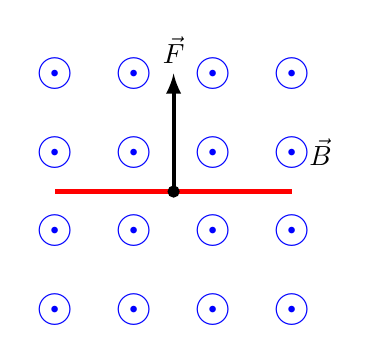
\begin{tikzpicture}
			\foreach \x in {0,1,...,3}{
				\foreach \y in {0,1,...,3}{
					\node[blue] at (\x,\y) {\LARGE$\odot$};}}
			\draw[line width=1.5pt, -latex] (1.5,1.5)--(1.5,3);
			\draw[line width=1.5pt,red] (0,1.5)--(3,1.5);
			\node[above] at (1.5,3) {$\vec{F}$};
			\node[right] at (3.1,2) {$\vec{B}$};
			\filldraw[black] (1.5,1.5) circle (2pt);
		\end{tikzpicture}
		&
		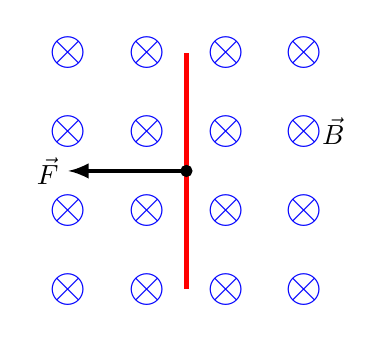
\begin{tikzpicture}
			\foreach \x in {0,1,...,3}{
				\foreach \y in {0,1,...,3}{
					\node[blue] at (\x,\y) {\LARGE$\otimes$};}}
			\draw[line width=1.5pt, -latex] (1.5,1.5)--(0,1.5);
			\draw[line width=1.5pt,red] (1.5,0)--(1.5,3);
			\node[left] at (0,1.5) {$\vec{F}$};
			\node[right] at (3.1,2) {$\vec{B}$};
			\filldraw[black] (1.5,1.5) circle (2pt);
		\end{tikzpicture}\\
		Hình a & Hình b
	\end{longtable}
\end{center}
\loigiai{
	\begin{center}
		\begin{longtable}{M{8cm}M{8cm}}
			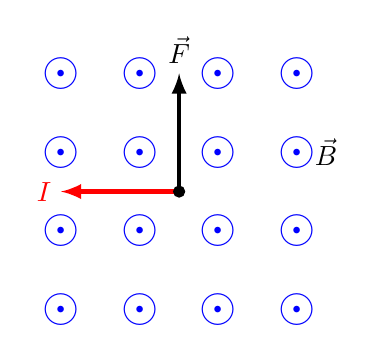
\begin{tikzpicture}
				\foreach \x in {0,1,...,3}{
					\foreach \y in {0,1,...,3}{
						\node[blue] at (\x,\y) {\LARGE$\odot$};}}
				\draw[line width=1.5pt, -latex] (1.5,1.5)--(1.5,3);
				\draw[line width=1.5pt,red, -latex] (1.5,1.5)--(0,1.5);
				\node[above] at (1.5,3) {$\vec{F}$};
				\node[left,red] at (0,1.5) {$I$};
				\node[right] at (3.1,2) {$\vec{B}$};
				\filldraw[black] (1.5,1.5) circle (2pt);
			\end{tikzpicture}
			&
			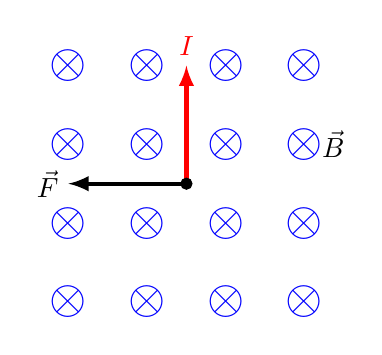
\begin{tikzpicture}
				\foreach \x in {0,1,...,3}{
					\foreach \y in {0,1,...,3}{
						\node[blue] at (\x,\y) {\LARGE$\otimes$};}}
				\draw[line width=1.5pt, -latex] (1.5,1.5)--(0,1.5);
				\node[left] at (0,1.5) {$\vec{F}$};
				\node[right] at (3.1,2) {$\vec{B}$};
				\draw[line width=1.5pt,red, -latex] (1.5,1.5)--(1.5,3);
				\node[above,red] at (1.5,3) {$I$};
				\filldraw[black] (1.5,1.5) circle (2pt);
			\end{tikzpicture}\\
			Hình a & Hình b
		\end{longtable}
	\end{center}}
\end{vd}
\begin{dang}{Vận dụng được biểu thức tính độ lớn lực từ }
	Lực từ tác dụng lên đoạn dây dẫn chiều dài $L$ đặt trong từ trường đều $B$ có dòng điên $I$ chạy qua:
	$$F=ILB\sin\theta.$$
	\end{dang}
\begin{vd}
	Một dòng điện có cường độ $\SI{0.6}{\ampere}$ chạy dọc theo dây dẫn bằng đồng được uốn thành khung hình tam giác ABC như hình vẽ. Khung được đặt trong từ trường đều có cảm ứng từ $\SI{2.8E-4}{\tesla}$. Xác định lực từ tác dụng lên cạnh:
	\begin{center}
		\begin{tikzpicture}
			\foreach \i in {0,1,...,5}
			\draw[blue, line width=1pt, decoration={markings, mark=at position 0.15 with {\arrow{stealth}}}, postaction={decorate}] (0, -0.5+\i)--(6,-0.5+\i);
			\coordinate (A) at (1.5,0);
			\coordinate (B) at (1.5,4);
			\coordinate (C) at (4.5,4);
			\coordinate (D) at (1.7,0);
			\draw[line width=1.5pt] (A)--(B)--(C)--(D)--($(D)-(0,0.5)$);
			\draw[line width=1.5pt,-latex] ($(A)-(0,0.5)$)--($(A)+(0,1)$);
			\node[below, left] at (A) {A};
			\node[above] at (B) {B};
			\node[above] at (C) {C};
			\node[above, blue] at (1,4.5) {$\vec{B}$};
			\node[left] at (1.5,1) {$I$};
			\node[below, left] at (A) {A};
			\node[left] at ($(A)!0.5!(B)$) {$\SI{40}{\centi\meter}$};
			\node[above] at ($(B)!0.5!(C)$) {$\SI{30}{\centi\meter}$};
			\node[right] at ($(C)!0.5!(D)$) {$\SI{50}{\centi\meter}$};
		\end{tikzpicture}
	\end{center}
	\begin{enumerate}[label=\alph*)]
		\item AB.
		\item AC.
		\item BC.
	\end{enumerate}
	\loigiai{
		\begin{center}
			\begin{tikzpicture}
				\foreach \i in {0,1,...,5}
				\draw[blue, line width=1pt, decoration={markings, mark=at position 0.15 with {\arrow{stealth}}}, postaction={decorate}] (0, -0.5+\i)--(6,-0.5+\i);
				\coordinate (A) at (1.5,0);
				\coordinate (B) at (1.5,4);
				\coordinate (C) at (4.5,4);
				\coordinate (D) at (1.7,0);
				\draw[line width=1.5pt] (A)--(B)--(C)--(D)--($(D)-(0,0.5)$);
				\draw[line width=1.5pt,-latex] ($(A)-(0,0.5)$)--($(A)+(0,1)$);
				\node[below, left] at (A) {A};
				\node[above] at (B) {B};
				\node[above] at (C) {C};
				\node[above, blue] at (1,4.5) {$\vec{B}$};
				\node[below, left] at (A) {A};
				\node[circle,red,fill=white,inner sep=0pt,minimum size=0pt,] at ($(A)!0.5!(B)$) {\LARGE$\otimes$};
				\node[circle,red,fill=white,inner sep=0pt,minimum size=0pt,] at ($(C)!0.5!(D)$) {\LARGE$\odot$};
				\node[red,left] at ($(A)!0.5!(B)-(0.25,0)$) {$\vec{F}_\text{AB}$};
				\node[red,right] at ($(C)!0.5!(D)+(0.25,0)$) {$\vec{F}_\text{CA}$};
			\end{tikzpicture}
		\end{center}	
		\begin{enumerate}[label=\alph*)]
			\item Độ lớn lực từ tác dụng lên cạnh AB:
			$$F_\text{AB}=IB\cdot\text{AB}\cdot\sin\left(\overrightarrow{\text{AB}},\vec{B}\right)=\left(\SI{0.6}{\ampere}\right)\cdot\left(\SI{2.8E-4}{\tesla}\right)\cdot\left(\SI{0.4}{\meter}\right)\cdot\sin\SI{90}{\degree}=\SI{6.72E-5}{\newton}.$$
			Chiều lực từ hướng vuông góc từ ngoài vào trong trang giấy.
			\item Độ lớn lực từ tác dụng lên cạnh AC:
			$$F_\text{CA}=IB\cdot\text{CA}\cdot\sin\left(\overrightarrow{\text{CA}},\vec{B}\right)=IB\cdot\text{CA}\cdot\sin\left(\pi -\widehat{BCA}\right)$$
			$$\Rightarrow F_\text{CA}=I\cdot B\cdot\text{CA}\cdot\sin\widehat{BCA}=IB\cdot\text{CA}\cdot\dfrac{\text{AB}}{\text{CA}}=\left(\SI{0.6}{\ampere}\right)\cdot\left(\SI{2.8E-4}{\tesla}\right)\cdot\left(\SI{0.5}{\meter}\right)\cdot\left(\dfrac{\SI{40}{\centi\meter}}{\SI{50}{\centi\meter}}\right)=\SI{6.72E-5}{\newton}.$$
			Chiều lực từ hướng vuông góc từ trong ra ngoài trang giấy.
			\item $F_\text{BC}=0$ vì $\left(\overrightarrow{\text{BC}},\vec{B}\right)=\SI{0}{\degree}$.
		\end{enumerate}
	}
\end{vd}

\begin{vd}
	Một dây dẫn thẳng MN chiều dài $\ell$, khối lượng của một đơn vị dài của dây là $d=\SI{0.04}{\kilogram/\meter}$. Dây dẫn được treo bằng hai dây dẫn nhẹ thẳng đứng và đặt trong từ trường đều có $\vec{B}$ vuông góc với mặt phẳng chứa MN và dây treo như hình bên dưới, độ lớn $B=\SI{0.04}{\tesla}$. Cho dòng điện có cường độ $I$ đi qua dây dẫn.
	\begin{center}
		\begin{tikzpicture}
			\coordinate (A) at (0,0);
			\coordinate (B) at (4,0);
			\coordinate (C) at (2,-4);
			\draw[line width=1pt] (A)--($(A)-(0,4)$);
			\draw[line width=1pt] (B)--($(B)-(0,4)$);
			\node[draw, line width=1pt, fill=black, shape=rectangle, minimum width=0.8cm, minimum height=0.3cm, anchor=center] at (A) {};
			\node[draw, line width=1pt, fill=black, shape=rectangle, minimum width=0.8cm, minimum height=0.3cm, anchor=center] at (B) {};
			\node[draw, line width=1pt, fill=orange!90!black, shape=rectangle, minimum width=5cm, minimum height=0.4cm, anchor=center] at (C) {};
			\node[below] at ($(A)+(-0.5,-4.25)$) {M};
			\node[below] at ($(B)+(0.5,-4.25)$) {N};
			\node[below] at ($(A)!0.5!(B)-(0,4.25)$) {$\ell$};
			\node[red] at ($(A)!0.5!(B)-(0,2)$) {\LARGE$\otimes$};
			\node[red, right] at ($(A)!0.5!(B)-(-0.25,2)$) {$\vec{B}$};
			
			
		\end{tikzpicture}
	\end{center}
	\begin{enumerate}[label=\alph*)]
		\item Xác định chiều và độ lớn của $I$ để lực căng của các dây treo bằng 0.
		\item Cho $\text{MN}=\SI{25}{\centi\meter}$, dòng điện qua dây dẫn có cường độ $I'=\SI{16}{\ampere}$ và có chiều từ N đến M. Tính lực căng mỗi dây trong trường hợp này. Lấy $g=\SI{10}{\meter/\second^2}$.
	\end{enumerate}
	\loigiai{Khối lượng dây $m=d\cdot\ell$.
		\begin{enumerate}[label=\alph*)]
			\item Để lực căng của các dây treo bằng 0 thì lực từ $\vec{F}$ phải cùng phương, ngược chiều và bằng về độ lớn với trọng lượng $\vec{P}$ như hình vẽ.\\\
			\begin{minipage}{0.6\textwidth}
				Áp dụng quy tắc bàn tay trái, để lực từ $\vec{F}$ cùng phương, ngược chiều $\vec{P}$ thì chiều dòng điện phải đi từ M đến N.\\
				Từ $F=P\Leftrightarrow I\ell B=mg$
				$$\Leftrightarrow I=\dfrac{mg}{B\ell}=\dfrac{gd}{B}=\dfrac{\left(\SI{0.04}{\kilogram/\meter}\right)\cdot\left(\SI{10}{\meter/\second^2}\right)}{\SI{0.04}{\tesla}}=\SI{10}{\ampere}.$$
			\end{minipage}
			\hfill
			\begin{minipage}{0.4\textwidth}
				\centering
				\begin{tikzpicture}
					\coordinate (A) at (0,0);
					\coordinate (B) at (3,0);
					\coordinate (C) at ($(A)!0.5!(B)-(0,3)$);
					\draw[line width=1pt] (A)--($(A)-(0,3)$);
					\draw[line width=1pt] (B)--($(B)-(0,3)$);
					\node[draw, line width=1pt, fill=black, shape=rectangle, minimum width=0.8cm, minimum height=0.3cm, anchor=center] at (A) {};
					\node[draw, line width=1pt, fill=black, shape=rectangle, minimum width=0.8cm, minimum height=0.3cm, anchor=center] at (B) {};
					\node[draw, line width=1pt, fill=orange!90!black, shape=rectangle, minimum width=4cm, minimum height=0.4cm, anchor=center] at (C) {};
					\node[below] at ($(A)+(-0.5,-3.25)$) {M};
					\node[below] at ($(B)+(0.5,-3.25)$) {N};
					\node[red] at ($(A)!0.5!(B)-(0,0.5)$) {\LARGE$\otimes$};
					\node[red, right] at ($(A)!0.5!(B)-(-0.25,0.5)$) {$\vec{B}$};
					
					\filldraw[black] (C) circle (2pt);
					\draw[-stealth, green!75!black, line width=1.5pt] (C)--($(C)+(0,1.5)$);
					\draw[-stealth, green!75!black,line width=1.5pt] (C)--($(C)-(0,1.5)$);
					\node[right, green!75!black] at ($(C)+(0,1.5)$) {$\vec{F}$};
					\node[right, green!75!black] at ($(C)+(0,-1.5)$) {$\vec{P}$};
				\end{tikzpicture}
			\end{minipage}
			\item Khi $I'=\SI{16}{\ampere}$, ta có:\\
			\begin{minipage}{0.6\textwidth}
				\begin{itemize}
					\item Lực từ $\vec{F}$ tác dụng lên thanh có độ lớn:
					$$F'=I'\ell B=\SI{0.16}{\newton}.$$
					\item Khối lượng dây:
					$$m=\ell d=\SI{0.01}{\kilogram}.$$
					\item Trọng lượng của thanh:
					$$P=mg=\SI{0.1}{\newton}.$$
				\end{itemize}
				Do $I'$ có chiều từ N đến M nên $\vec{F}'$ cùng phương, cùng chiều với $\vec{P}$.\\
				$\Rightarrow$ Lực căng mỗi dây: $T=\dfrac{P+F'}{2}=\SI{0.13}{\newton}.$
			\end{minipage}
			\hfill
			\begin{minipage}{0.4\textwidth}
				\centering
				\begin{tikzpicture}
					\coordinate (A) at (0,0);
					\coordinate (B) at (3,0);
					\coordinate (C) at ($(A)!0.5!(B)-(0,3)$);
					\draw[line width=1pt] (A)--($(A)-(0,3)$);
					\draw[line width=1pt] (B)--($(B)-(0,3)$);
					\draw[purple, line width=1.5pt,-stealth] ($(A)-(0,3)$)--($(A)-(0,1.5)$);
					\draw[purple, line width=1.5pt,-stealth] ($(B)-(0,3)$)--($(B)-(0,1.5)$);
					\node[draw, line width=1pt, fill=black, shape=rectangle, minimum width=0.8cm, minimum height=0.3cm, anchor=center] at (A) {};
					\node[draw, line width=1pt, fill=black, shape=rectangle, minimum width=0.8cm, minimum height=0.3cm, anchor=center] at (B) {};
					\node[draw, line width=1pt, fill=orange!90!black, shape=rectangle, minimum width=4cm, minimum height=0.4cm, anchor=center] at (C) {};
					\node[below] at ($(A)+(-0.5,-3.25)$) {M};
					\node[below] at ($(B)+(0.5,-3.25)$) {N};
					\node[red] at ($(A)!0.5!(B)-(0,0.5)$) {\LARGE$\otimes$};
					\node[red, right] at ($(A)!0.5!(B)-(-0.25,0.5)$) {$\vec{B}$};
					
					\filldraw[black] (C) circle (2pt);
					\draw[-stealth, blue, line width=1.5pt] (C)--($(C)+(0,-2)$);
					\draw[-stealth, green!75!black,line width=1.5pt] (C)--($(C)-(0,1.5)$);
					\node[right, blue] at ($(C)+(0,-2)$) {$\vec{F}'$};
					\node[right, green!75!black] at ($(C)+(0,-1.5)$) {$\vec{P}$};
					\node[right, purple] at ($(B)-(0,1.5)$) {$\vec{T}$};
					\node[left, purple] at ($(A)-(0,1.5)$) {$\vec{T}$};
				\end{tikzpicture}
			\end{minipage}
		\end{enumerate}
		
	}
\end{vd}
\begin{vd}
	Treo đoạn dây dẫn $\text{MN}=\SI{5}{\centi\meter}$ khối lượng $\SI{5}{\gram}$ bằng hai dây không dãn, khối lượng không đáng kể. Không gian có từ trường đều với vector cảm ứng từ có phương vuông góc với đoạn dây, chiều từ trên xuống và có độ lớn $B=\SI{0.5}{\tesla}$. Tính góc lệch của dây treo so với phương thẳng đứng khi đoạn dây MN nằm cân bằng, biết cường độ dòng điện qua đoạn dây MN là $\SI{2}{\ampere}$, lấy $g=\SI{10}{\meter/\second^2}$.
	\begin{center}
		\begin{tikzpicture}
			\coordinate (A) at (0,0);
			\coordinate (B) at (4,0);
			\coordinate (C) at (2,-4);
			\draw[line width=1pt] (A)--($(A)-(0,4)$);
			\draw[line width=1pt] (B)--($(B)-(0,4)$);
			\node[draw, line width=1pt, fill=black, shape=rectangle, minimum width=0.8cm, minimum height=0.3cm, anchor=center] at (A) {};
			\node[draw, line width=1pt, fill=black, shape=rectangle, minimum width=0.8cm, minimum height=0.3cm, anchor=center] at (B) {};
			\node[draw, line width=1pt, fill=orange!90!black, shape=rectangle, minimum width=5cm, minimum height=0.4cm, anchor=center] at (C) {};
			\node[below] at ($(A)+(-0.5,-4.25)$) {M};
			\node[below] at ($(B)+(0.5,-4.25)$) {N};
			\node[below] at ($(A)!0.5!(B)-(0,4.25)$) {$\ell$};
			\node[red, right] at ($(A)!0.5!(B)-(0,2.5)$) {$\vec{B}$};
			\draw[-stealth, red, line width=1.5pt] ($(A)!0.5!(B)-(0,1)$)--($(A)!0.5!(B)-(0,2.5)$);
			
		\end{tikzpicture}
	\end{center}
	\loigiai{
		\begin{center}
			\begin{tikzpicture}
				\coordinate (O) at(0,0);
				\coordinate (A) at (-45:4);
				\coordinate (B) at (-90:4);
				\node[draw, line width=1pt, fill=black, shape=rectangle, minimum width=1cm, minimum height=0.3cm, anchor=center] at (O) {};
				\draw[line width=1.5pt] (O)--(A);
				\draw[line width=1.5pt, dashed] (O)--(B);
				\draw[line width=1.5pt, -stealth, blue] (A)--($(A)-(0,1.5)$);
				\draw[line width=1.5pt, -stealth, red] (A)--($(A)+(1.5,0)$);
				\draw[line width=1.5pt, -stealth, green!60!black] (A)--($(A)+(135:1.5)$);
				\draw[-stealth, red, line width=1.5pt] (-0.5,-0.5)--(-0.5,-2.5);
				\node[red,left] at (-0.5,-2.5) {$\vec{B}$};
				\node[circle,red,fill=white,inner sep=0pt,minimum size=0pt,] at (A) {\LARGE$\odot$};
				\node[green!60!black, above right] at ($(A)+(135:1.5)$) {$\vec{T}$};
				\node[blue, right] at ($(A)-(0,1.5)$) {$\vec{P}$};
				\node[red, above] at ($(A)+(1.5,0)$) {$\vec{F}$};
				\tkzMarkAngle[color=black, line width=1.25pt](B,O,A);
				\tkzLabelAngle[color=black,pos=1.2](B,O,A){$\alpha$}
			\end{tikzpicture}
		\end{center}
		Dây dẫn nằm cân bằng nên:
		$$\vec{P}+\vec{F}+\vec{T}=\vec{0}$$
		Từ đó, ta có:
		$$\tan\alpha=\dfrac{F}{P}=\dfrac{I\ell B\sin\SI{90}{\degree}}{mg}=1\Rightarrow \alpha=\SI{45}{\degree}.$$
	}
\end{vd}
\subsection{Bài tập}
\subsubsection{Trắc nghiệm nhiều phương án lựa chọn}
\setcounter{ex}{0}
\Opensolutionfile{ans}[ans/VN12-Y24-PH-SYL-018P-TN]
% ===================================================================
\begin{ex}
	Cho các phát biểu sau đây:
	\begin{enumerate}[label=(\arabic*)]
		\item Từ trường có thể tác dụng lực từ lên các điện tích đứng yên đặt trong nó.
		\item Từ trường có khả năng tác dụng lực từ lên dòng điện đặt trong nó.
		\item Từ trường có khả năng tác dụng lực từ lên nam châm đặt trong nó.
		\item Đường sức từ luôn là những đường cong khép kín.
	\end{enumerate}	
	Trong các phát biểu trên, số phát biểu đúng là
	\choice
	{1}
	{2}
	{\True 3}
	{4}
	\loigiai{Các phát biểu đúng là (2), (3), (4)}
\end{ex}

% ===================================================================
\begin{ex}
	Trong hệ SI, đơn vị đo độ lớn cảm ứng từ là 	
	\choice
	{fara $\left(\si{\farad}\right)$}
	{henry $\left(\si{\ohm}\right)$}
	{\True tesla $\left(\si{\tesla}\right)$}
	{ampere $\left(\si{\ampere}\right)$}
	\loigiai{}
\end{ex}
% ===================================================================
\begin{ex}
	Đặt một dây dẫn có chiều dài là $\ell$, mang dòng điện $I$ trong từ trường đều có độ lớn cảm ứng từ $B$ và tạo với cảm ứng từ góc $\theta$. Lực do từ trường tác dụng lên dây dẫn có độ lớn là
	\choice
	{$\dfrac{I\ell}{B}\sin\theta$}
	{$BI\ell \cos\theta$}
	{\True $BI\ell\sin\theta$}
	{$I^2\ell B\sin\theta$}
	\loigiai{}
\end{ex}



% ===================================================================
\begin{ex}
	Chọn cụm từ và công thức phù hợp để điền vào chỗ trống.\\
	Cảm ứng từ là một đại lượng (1)\dots, đặc trưng cho từ trường về phương diện tác dụng lực. Khi một đoạn dây dẫn thẳng có chiều dài $L$, mang dòng điện có cường độ $I$ được đặt trong vùng từ trường đều có cảm ứng từ $\vec{B}$ hợp với chiều dòng điện một góc $\theta$ thì độ lớn cảm ứng từ được xác định bởi biểu thức (2) \dots
	\choice
	{(1) vô hướng, (2) $B=\dfrac{F}{IL\cos\theta}$}
	{\True (1) vector, (2) $B=\dfrac{F}{IL\sin\theta}$}
	{(1) vô hướng, (2) $B=\dfrac{F}{IL\sin\theta}$}
	{(1) vector, (2) $B=\dfrac{F}{IL\cos\theta}$}
	\loigiai{}
\end{ex}
% ===================================================================
\begin{ex}
	Tìm phát biểu \textbf{đúng} trong các phát biểu sau.\\
	Một dòng điện đặt vuông góc với đường sức từ trong từ trường, chiều của lực từ tác dụng vào dòng điện sẽ không thay đổi khi
	\choice
	{đổi chiều dòng điện ngược lại}
	{đổi chiều cảm ứng từ ngược lại}
	{\True đồng thời đổi chiều dòng điện và đổi chiều cảm ứng từ}
	{quay dòng điện một góc $90^{\circ}$ xung quanh đường sức từ}
	\loigiai{}
\end{ex}
% ===================================================================
\begin{ex}
	Chỉ ra phát biểu \textbf{sai}.
	\choice
	{Lực từ tác dụng lên đoạn dây dẫn mang dòng điện có phương vuông góc với dòng điện}
	{Lực từ tác dụng lên đoạn dây dẫn mang dòng điện có phương vuông góc với đường cảm ứng từ}
	{\True Lực từ tác dụng lên đoạn dây dẫn mang dòng điện có phương vuông góc với mặt phẳng chứa dòng điện và đường cảm ứng từ}
	{Lực từ tác dụng lên đoạn dây dẫn mang dòng điện có phương tiếp tuyến với các đường cảm ứng từ}
	\loigiai{}
\end{ex}
% ===================================================================
\begin{ex}
	Phát biểu nào sau đây \textbf{không đúng}?	
	\choice
	{Lực từ tác dụng lên một đoạn dây dẫn mang dòng điện đặt trong từ trường đều tỉ lệ thuận với cường độ dòng điện chạy qua đoạn dây dẫn}
	{Lực từ tác dụng lên một đoạn dây dẫn mang dòng điện đặt trong từ trường đều tỉ lệ thuận với chiều dài của đoạn dây dẫn}
	{Lực từ tác dụng lên một đoạn dây dẫn mang dòng điện đặt trong từ trường đều tỉ lệ thuận với cảm ứng từ tại điểm đặt đoạn dây dẫn}
	{\True Lực từ tác dụng lên một đoạn dây dẫn mang dòng điện đặt trong từ trường đều tỉ lệ thuận với góc hợp bởi đoạn dây dẫn và đường sức từ}
	\loigiai{$$F=ILB\sin\theta.$$}
\end{ex}
% ===================================================================
\begin{ex}
	Phát biểu nào dưới đây \textbf{đúng}?\\
	Cho một đoạn dây dẫn mang dòng điện $I$ đặt song song với đường sức từ, chiều của dòng điện ngược chiều với chiều của đường sức từ.
	\choice
	{\True Lực từ luôn bằng không khi tăng cường độ dòng điện}
	{Lực từ tăng khi tăng cường độ dòng điện}
	{Lực từ giảm khi tăng cường độ dòng điện}
	{Lực từ đổi chiều khi ta đổi chiều dòng điện}
	\loigiai{}
\end{ex}
% ===================================================================
\begin{ex}
	Một dây dẫn được đặt nằm ngang theo hướng nam bắc trong một từ trường đều có cảm ứng từ nằm ngang hướng về phía đông. Trong dây dẫn có dòng electron chuyển động theo chiều về phía nam. Phát biểu nào sau đây là \textbf{đúng}?
	\choice
	{Lực tác dụng lên dây có hướng là hướng đông}
	{\True Lực tác dụng lên dây có hướng vuông góc và đi vào trang giấy}
	{Lực tác dụng lên dây có hướng vuông góc và ra khỏi trang giấy}
	{Không có lực từ tác dụng lên dây}
	\loigiai{}
\end{ex}
% ===================================================================
\begin{ex}
	Khi sét đánh, có dòng điện tích âm chuyển động từ đám mây xuống mặt đất. Từ trường của Trái Đất hướng về phía bắc. Tia sét bị từ trường Trái Đất làm chệch hướng theo hướng nào?
	
	\choice
	{Bắc}
	{Nam}
	{Đông}
	{\True Tây}
	\loigiai{Áp dụng quy tắc bàn tay trái, từ trường hướng về phía Bắc, dòng điện gây ra bởi tia sét hướng lên trên $\Rightarrow$ lực từ tác dụng lên tia sét hướng về phía Tây.}
\end{ex}

% ===================================================================
\begin{ex}
	Hai dây dẫn thẳng, dài, đặt vuông góc với nhau, rất gần nhau nhưng không chạm vào nhau. Dòng điện qua hai dây dẫn có chiều như hình vẽ và có cùng cường độ. Từ trường do hai dây dẫn gây ra có thể triệt tiêu nhau trong vùng nào?
	\begin{center}
		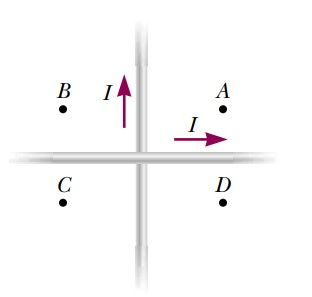
\includegraphics[width=0.3\linewidth]{figs/VN12-Y24-PH-SYL-017P-8}
	\end{center}
	\choice
	{vùng A và D}
	{\True vùng A và C}
	{vùng B và D}
	{vùng B và C}
	\loigiai{}
\end{ex}
% ===================================================================
\begin{ex}
	Xét dây dẫn có chiều dài $L$, có dòng điện $I$ chạy qua đặt tại điểm M trong từ trường đều, chịu tác dụng của lực điện từ $F$. Khi thay đổi $L$ hoặc $I$ thì $F$ thay đổi nhưng tỉ số nào sau đây luôn không đổi?
	\choice
	{$\frac{FI}{2L}$}
	{\True $\frac{F}{IL}$}
	{$\frac{FL}{I}$}
	{$\frac{FI^2}{L}$}
	\loigiai{}
\end{ex}
% ===================================================================
\begin{ex}
	Một đoạn dây dẫn đặt trong từ trường đều. Nếu chiều dài dây dẫn và cường độ dòng điện qua dây dẫn tăng 2 lần thì độ lớn lực từ tác dụng lên dây dẫn	
	\choice
	{tăng 2 lần}
	{giảm 2 lần}
	{\True tăng 4 lần}
	{không đổi}
	\loigiai{
		$$F=ILB\sin\theta.$$
	}
\end{ex}

% ===================================================================
\begin{ex}
	Một đoạn dây dẫn mang dòng điện được đặt vuông góc với từ trường đều có cảm ứng từ $B$. Khi dòng điện trong dây là $I$ thì lực từ tác dụng lên đoạn dây đó là $F$. Cũng đoạn dây đó, cho dòng điện chạy qua dây là $0,25I$ và đặt trong từ trường $2B$, lực từ tác dụng lên đoạn dây đó là
	\choice
	{$\dfrac{F}{4}$}
	{\True $\dfrac{F}{2}$}
	{$F$}
	{$2F$}
	\loigiai{}
\end{ex}
% ===================================================================
\begin{ex}
	Trong thí nghiệm đo độ lớn cảm ứng từ bằng "cân dòng điện" với bố trí thí nghiệm được thể hiện như trong hình \ref{fig:18P-11}, khung dây được sử dụng có kích thước là $\SI{100}{\milli\meter}\times\SI{80}{\milli\meter}$ như hình \ref{fig:18P-12}. Nếu ta thay khung dây ban đầu thành một khung dây khác có kích thước là $\SI{100}{\milli\meter}\times\SI{20}{\milli\meter}$ nhưng vẫn giữ nguyên góc hợp bởi mặt phẳng khung dây và các đường sức từ cũng như cường độ dòng điện qua khung dây và nam châm điện thì nhận định nào sau đây về lực từ do từ trường tác dụng lên khung dây là \textbf{đúng}?
	\begin{center}
		\begin{tabular}{M{8cm}M{8cm}}
			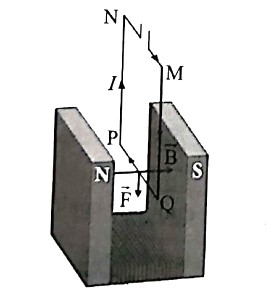
\includegraphics[width=0.6\linewidth]{figs/VN12-Y24-PH-SYL-018P-11}
			\captionof{figure}{}
			\label{fig:18P-11}
			&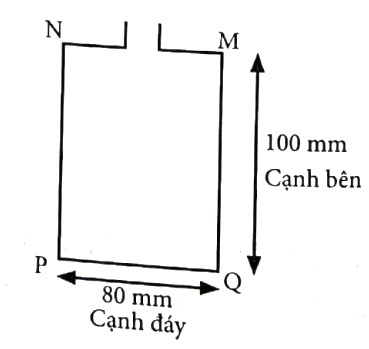
\includegraphics[width=0.6\linewidth]{figs/VN12-Y24-PH-SYL-018P-12}
			\captionof{figure}{}
			\label{fig:18P-12}
		\end{tabular}
	\end{center}
	\choice
	{Không đổi chiều và độ lớn tăng 4 lần}
	{\True Không đổi chiều và độ lớn giảm 4 lần}
	{Đổi chiều và độ lớn giảm 4 lần}
	{Đổi chiều và độ lớn tăng 4 lần}
	\loigiai{
		Vi từ trường chỉ tác dụng lực lên cạnh dưới của khung và độ lớn của lực từ được xác định bằng biểu thức $F=B I L$ nên khi chiều dài cạnh đáy giảm 4 lần thì độ lớn lực từ giảm 4 lần.
	}
\end{ex}


% ===================================================================
\begin{ex}
	Một đoạn dây dẫn dài $\ell=\SI{0.8}{\meter}$ đặt trong từ trường đều sao cho dây dẫn hợp với vector cảm ứng từ một góc $\SI{60}{\degree}$. Biết dòng điện $I=\SI{20}{\ampere}$ và dây dẫn chịu một lực là $F=\SI{2E-2}{\newton}$. Độ lớn của cảm ứng từ là
	\choice
	{$\SI{0.8E-3}{\tesla}$}
	{$\SI{E-3}{\tesla}$}
	{\True $\SI{1.4E-3}{\tesla}$}
	{$\SI{1.6E-3}{\tesla}$}
	\loigiai{
		$$B=\dfrac{F}{I\ell\sin\theta}=\dfrac{\SI{2E-2}{\newton}}{\left(\SI{20}{\ampere}\right)\cdot\left(\SI{0.8}{\meter}\right)\cdot\sin\SI{60}{\degree}}\approx\SI{1.44E-3}{\tesla}.$$
	}
\end{ex}

% ===================================================================
\begin{ex}
	Một đoạn dây dẫn dài $\SI{2}{\centi\meter}$ nằm trong từ trường, dòng điện chạy qua có cường độ $\SI{1}{\ampere}$. Một nam châm tạo từ trường có cường độ cảm ứng từ $\SI{0.5}{\tesla}$ và hợp với dây dẫn một góc $\SI{30}{\degree}$. Lực từ tác dụng lên dây dẫn có độ lớn là
	
	\choice
	{$\SI{10E-2}{\newton}$}
	{$\SI{1E-2}{\newton}$}
	{\True $\SI{0.5E-2}{\newton}$}
	{$\SI{50E-2}{\newton}$}
	\loigiai{
		$$
		F=BIL\sin \alpha=\SI{0.5E-2}{\newton}.
		$$
		
	}
\end{ex}
% ===================================================================
\begin{ex}
	Khi góc hợp bởi vector cảm ứng từ với đoạn dây dẫn có dòng điện là $\alpha=\SI{90}{\degree}$ thì lực từ tác dụng có giá trị là $\SI{0.4}{\newton}$. Nếu thay đổi góc $\alpha$ nhỏ dần đến $\SI{0}{\degree}$, thì lực tác dụng thay đổi như thế nào?
	\choice
	{\True Lực cũng giảm dần đến 0}
	{Lực tăng lên đến $\SI{0.8}{\newton}$}
	{Lực không đổi}
	{Lực giảm xuống $\SI{0.2}{\newton}$}
	\loigiai{}
\end{ex}

% ===================================================================
\begin{ex}
	Một dây dẫn thẳng có chiều dài $\SI{3.0}{\meter}$ mang dòng điện $\SI{6.0}{\ampere}$ được đặt nằm ngang, hướng của dòng điện tạo với hướng bắc một góc $\SI{50}{\degree}$ lệch về phía tây. Tại điểm này, cảm ứng từ của từ trường Trái Đất có độ lớn là $\SI{0.14E-4}{\tesla}$ và hướng bắc. Lực tác dụng lên dây có độ lớn là
	\choice
	{$\SI{0.28E-4}{\newton}$}
	{$\SI{2.5E-4}{\newton}$}
	{$\SI{1.9E-4}{\newton}$}
	{\True $\SI{1.6E-4}{\newton}$}
	\loigiai{
		$$F=ILB\sin\SI{50}{\degree}\approx\SI{1.6E-4}{\newton}.$$	
	}
\end{ex}
% ===================================================================
\begin{ex}
	Một dây đồng dài $\SI{25}{\centi\meter}$, có khối lượng là $\SI{10}{\gram}$ nằm trong từ trường $\SI{0.20}{\tesla}$. Lấy gia tốc trọng trường $g=\SI{10}{\meter/\second^2}$. Cường độ dòng điện nhỏ nhất chạy qua dây gây ra lực từ có độ lớn bằng trọng lượng của dây là
	\choice
	{$\SI{1.3}{\ampere}$}
	{$\SI{1.5}{\ampere}$}
	{\True $\SI{2.0}{\ampere}$}
	{$\SI{4.9}{\ampere}$}
	\loigiai{
		$$I_\text{min}=\dfrac{P}{BL\left(\sin\theta\right)_{\text{max}}}=\SI{2.0}{\ampere}.$$	
	}
\end{ex}
% ===================================================================
\begin{ex}
	Trong thí nghiệm xác định độ lớn cảm ứng từ của nam châm điện chữ $U$ bằng "cân dòng điện" (theo phương án thí nghiệm trong Bài 11 của SGK CTST), xét trạng thái ổn định với đòn cân nằm ngang cân bằng khi có dòng điện chạy trong khung dây và nam châm điện, góc hợp bởi mặt phẳng khung dây và các đường sức từ là $\SI{90}{\degree}$. Nếu ta làm khung dây bị lệch một góc nào đó so với vị trí ban đầu thì khi đòn cân được điều chỉnh trở về lại trạng thái nằm ngang cân bằng, số chỉ của lực kế sẽ	
	\choice
	{vẫn giữ nguyên giá trị ban đầu}
	{lớn hơn giá trị ban đầu}
	{\True nhỏ hơn giá trị ban đầu}
	{dao động xung quanh giá trị ban đầu}
	\loigiai{
		Vì độ lớn của lực từ được xác định bằng biểu thức $F=ILB\sin\theta$ nên khi khung dây bị lệch so với ban đầu thì $\sin\theta$ giảm dẫn đến $F$ giảm. Vì vậy số chỉ của lực kế giảm so với ban đầu.	
	}
\end{ex}


% ===================================================================
\begin{ex}
	Thanh dây dẫn thẳng MN có chiều dài $\SI{20}{\centi\meter}$, khối lượng $\SI{10}{\gram}$, được treo trên hai sợi dây mảnh sao cho MN nằm ngang. Cả hệ thống được đặt trong từ trường đều có cảm ứng từ $B=\SI{0.25}{\tesla}$ và vector $\vec{B}$ hướng lên trên theo phương thẳng đứng. Nếu cho dòng điện $I=\xsi{2\sqrt{3}}{\ampere}$ chạy qua, người ta thấy thanh MN được nâng lên vị trí cân bằng mới và hai sợi dây treo bây giờ lệch một góc $\alpha$ so với phương thẳng đứng. Cho $g=\SI{10}{\meter/\second^2}$, góc lệch $\alpha$ là	
	\begin{center}
		\begin{tikzpicture}
			\coordinate (A) at (0,0);
			\coordinate (B) at (3,1.5);
			\coordinate (A1) at ($(A)+(0,-1.5)$);
			\coordinate (B1) at ($(B)+(0,-1.5)$);
			\coordinate (M) at ($(A)+(-30:3)$);
			\coordinate (N) at ($(B)+(-30:3)$);
			\draw[line width=1pt] (A)--(M);
			\draw[line width=1pt] (B)--(N);
			\draw[line width=1pt, dashed] (A)--(A1);
			\draw[line width=1pt, dashed] (B)--(B1);
			\draw[line width=4pt] (M)--(N);
			\draw[line width=3pt, blue] (A)--+(30:0.5)--+(-150:0.5);
			\draw[line width=3pt, blue] (B)--+(30:0.5)--+(-150:0.5);
			\tkzMarkAngle[size=0.75cm,color=red](A1,A,M);
			\tkzLabelAngle[color=red,pos=1.2](A1,A,M){$\alpha$};
		\end{tikzpicture}
	\end{center}
	\choice
	{$\SI{30}{\degree}$}
	{$\SI{45}{\degree}$}
	{\True $\SI{60}{\degree}$}
	{$\SI{90}{\degree}$}
	\loigiai{}
\end{ex}

\Closesolutionfile{ans}

\subsubsection{Trắc nghiệm đúng/sai}
\Opensolutionfile{ans}[ans/VN12-Y24-PH-SYL-018P-TF]
\setcounter{ex}{0}
% ===================================================================
\begin{ex}
	Một thí nghiệm để tìm ra lực từ tác dụng lên một đoạn dây dẫn chứa dòng điện được đặt trong từ trường của một nam châm.
	\choiceTF[t]
	{\True Nếu cường độ dòng điện qua dây tăng lên, lực từ tác dụng lên dây sẽ tăng lên}
	{Nếu khoảng cách giữa dây dẫn và nam châm tăng lên, lực từ tác dụng lên dây sẽ tăng lên}
	{\True Lực từ chỉ có thể tác dụng lên dây dẫn khi có dòng điện chạy qua dây}
	{Độ lớn lực từ tác dụng lên đoạn dây dẫn sẽ thay đổi khi dòng điện chạy qua dây đảo chiều}
	\loigiai{}
\end{ex}
% ===================================================================
\begin{ex}
	Trong mỗi phát biểu sau, em hãy chọn đúng hoặc sai.	
	\choiceTF[t]
	{Cảm ứng từ là một đại lượng vô hướng}
	{\True Tiếp tuyến tại bất kì điểm nào trên đường sức từ đều có phương, chiều trùng với phương, chiều của vector cảm ứng từ tại điểm đó}
	{\True Từ trường ở vùng không gian giữa hai cực của nam châm chữ U được xem là từ trường đều}
	{Trong từ trường đều, các đường sức từ song song nhau nhưng vector cảm ứng từ tại các điểm khác nhau lại không bằng nhau về độ lớn}
	\loigiai{}
\end{ex}
% ===================================================================
\begin{ex}
	\immini{Xét một dây dẫn thẳng dài vô hạn có dòng điện cường độ $I$ chạy qua. Hai điểm M, N nằm trong cùng một mặt phẳng vuông góc với dây dẫn và cách đều dây dẫn, biết OM vuông góc với ON.\\
		Trong mỗi phát biểu sau về cảm ứng từ tại điểm M và N do dòng điện này gây ra, em hãy chọn đúng hoặc sai.	}
	{		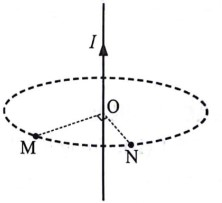
\includegraphics[width=0.4\linewidth]{figs/VN12-Y24-PH-SYL-018P-1}
	}
	
	\choiceTF[t]
	{\True Cảm ứng từ tại điểm M có phương vuông góc với OM}
	{cảm ứng từ tại điểm N song song với dây dẫn và có hướng cùng chiều với dòng điện chạy trong dây dẫn}
	{\True M và N cùng nằm trên một đường sức từ}
	{\True Cảm ứng từ tại M và N bằng nhau về độ lớn}
	\loigiai{}
\end{ex}

% ===================================================================
\begin{ex}
	Chỉ ra đáp án đúng, đáp án sai.
	\choiceTF[t]
	{\True Nam châm tác dụng lên dòng điện thực chất là tương tác giữa từ trường của nam châm với các electron của dây điện}
	{Nam châm tác dụng lên dòng điện thực chất là tương tác giữa từ trường của nam châm với từ trường do các electron chuyển động gây ra}
	{Phương của lực từ trùng với phương của dòng điện}
	{\True Lực từ tác dụng lên đoạn dây dẫn mang dòng điện có phương vuông góc với đoạn dây dẫn và vuông góc vector cảm ứng từ}
	\loigiai{}
\end{ex}
% ===================================================================
\begin{ex}
	Trong mỗi nhận định sau về thí nghiệm đo độ lớn cảm ứng từ bằng "cân dòng điện" với bố trí thí nghiệm được thể hiện như hình \ref{fig:18P-10}. Em hãy chọn đúng hoặc sai cho mỗi nhận định sau đây.
	\begin{center}
		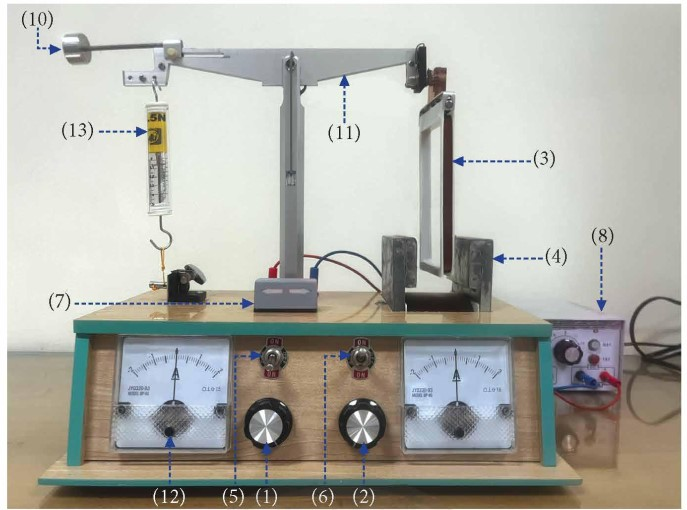
\includegraphics[width=0.55\linewidth]{figs/VN12-Y24-PH-SYL-018P-10}
		\captionof{figure}{Thí nghiệm đo độ lớn cảm ứng từ bằng "cân dòng điện"}
		\label{fig:18P-10}
	\end{center}
	\choiceTFt
	{\True Cơ sở lí thuyết của thí nghiệm này dựa trên tác dụng lực của từ trường đều lên đoạn dây dẫn có dòng điện chạy qua}
	{\True Trước khi bật công tắc cho dòng điện chạy qua khung dây dẫn và nam châm điện, cần phải điều chỉnh sao cho đòn cân nằm ngang rồi đọc giá trị của lực kế}
	{Khi đóng công tắc cho dòng điện chạy qua khung dây dẫn và nam châm điện, từ trường tạo ra bởi nam châm luôn tác dụng lực đẩy khung dây đi lên}
	{\True Trong thí nghiệm, từ trường tạo bởi nam châm điện không tác dụng lực từ lên các cạnh bên của khung dây}
	{Từ trường trong vùng không gian giữa hai nhánh của nam châm điện trong thí nghiệm được xem gần đúng là từ trường đều. Chiều và độ lớn của vector cảm ứng từ trong vùng từ trường này không phụ thuộc vào chiều và cường độ dòng điện chạy qua cuộn dây của nam châm}
	{Có thể lấy giá trị của lực kế khi đòn cân chưa nằm ngang ổn định}
	{\True Công dụng của các núm xoay (1) và (2) là điều chỉnh giá trị cường độ dòng điện chạy qua khung dây và cuộn dây của nam châm điện}
	{\True Có thể thay đổi chiều của lực từ tác dụng lên khung dây bằng việc sử dụng công tắc (5) hoặc (6)}
	\loigiai{}
\end{ex}

% ===================================================================
\begin{ex}
	Cho một khung dây dẫn hình chữ nhật có chiều rộng $\SI{20}{\centi\meter}$, mang dòng điện, đặt trong từ trường đều có cảm ứng từ $\vec{B}$ hướng vào trong như hình vẽ. Biết mặt phẳng vòng dây vuông góc với các đường sức từ. Bên ngoài vòng tròn, từ trường bằng 0.\begin{center}
		\begin{tikzpicture}
			\foreach \x in {-3,-2,...,3}{
				\foreach \y in {-3,-2,...,3}{
					\node[blue] at (\x,\y) {\LARGE$\odot$};
					
			}}
			\fill[white, even odd rule] (0,0) circle(3.4) (0,0) circle (4.5);
			\draw[dashed, line width=1pt] (0,0) circle (3.5);
			\draw[line width=1.5pt,decoration={markings, mark=at position 0.5 with {\arrow{stealth}}},postaction={decorate}
			] (-1.5,3.75)--(-1.5,0.65)--(1.5,0.65)--(1.5,3.75);
			\node[black] at (0,0.35) {$\SI{20}{\centi\meter}$};
		\end{tikzpicture}
	\end{center}
	\choiceTF[t]
	{\True Lực từ tổng hợp tác dụng lên khung dây hướng xuống dưới}
	{Nếu sử dụng dòng điện có cường độ $\SI{5.00}{\ampere}$ thì lực từ trên mỗi tesla tác dụng lên khung dây là $\SI{2.00}{\newton/\tesla}$}
	{Nếu ta quay khung dây $\SI{90}{\degree}$ để vector cảm  ứng từ song song mặt phẳng khung dây, lực từ tác dụng lên khung sẽ giảm xuống bằng 0}
	{\True Khi dòng điện qua khung dây đổi chiều, lực từ tổng hợp tác dụng lên khung dây sẽ đổi chiều}
	\loigiai{
		\begin{itemchoice}
			\itemch Đúng. Vì lực từ tổng hợp tác dụng lên hai đoạn dây thẳng đứng bị triệt tiêu, chỉ còn lực tác dụng lên đoạn dây dẫn nằm ngang và lực này hướng xuống dưới.
			\itemch Sai. Vì $\dfrac{F}{B}=IL\sin\SI{90}{\degree}=\SI{1}{\newton/\tesla}$.
				\itemch Sai. Lực từ tác dụng ở hai cạnh bên tạo thành ngẫu lực làm khung quay.
			\itemch Đúng. Hướng lực từ phụ thuộc vào hướng của dòng điện theo quy tắc bàn tay trái.
			
		\end{itemchoice}	
	}
\end{ex}
% ===================================================================
\begin{ex}
	Một đoạn dây thẳng bằng đồng được đặt vuông góc với từ trường đều, có dòng điện $\SI{7.0}{\ampere}$ chạy qua và nằm cân bằng trong từ trường. Khối lượng của một đơn vị chiều dài của đoạn dây là $\SI{46.6}{\gram/\meter}$, và gia tốc trọng trường là $\SI{9.8}{\meter/\second^2}$. Bỏ qua ảnh hường của từ trường Trái Đất lên đoạn dây.
	\begin{center}
		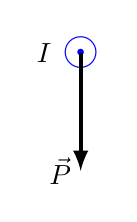
\begin{tikzpicture}
			\node[blue] at (0,0) {\LARGE$\odot$};
			\node[left] at (-0.25,0) {$I$};
			\draw[-latex, line width=1.5pt] (0,0)--+(0,-1.5);
			\node[left] at (0,-1.5) {$\vec{P}$};
		\end{tikzpicture}
	\end{center}
	\choiceTF[t]
	{\True Lực từ tác dụng lên đoạn dây sẽ tăng lên nếu cảm ứng từ trong từ trường đều tăng lên mà dòng điện giữ nguyên}
	{Cảm ứng từ $\vec{B}$ có phương nằm ngang và chiều từ phải sang trái}
	{\True Lực từ có thể cân bằng với trọng lực khi đoạn dây được đặt trong một từ trường với cảm ứng từ bằng $\SI{6.5E-2}{\tesla}$}
	{Nếu thay dây dẫn trên bằng dây dẫn nhôm có cùng kích cỡ nhưng khối lượng riêng thấp hơn, thì lực từ cần để cân bằng dây sẽ tăng}
	\loigiai{
		\begin{itemchoice}
			\itemch Đúng. Vì $F=ILB\sin\theta$.
			\itemch Sai. Áp dụng quy tắc bàn tay trái, cảm ứng từ có phương nằm ngang và chiều từ trái sang phải.
			\itemch Đúng. Khối lượng dây $m=\SI{46.6E-3}{}\cdot\ell$.\\
			Lực từ và trọng lực có thể cân bằng nhau nếu cảm ứng từ $B$ được điều chỉnh sao cho
			$$F=P\Leftrightarrow mg=I\ell B\Rightarrow B=\dfrac{m}{\ell}\cdot\dfrac{g}{I}=\SI{6.5E-2}{\tesla}.$$
			\itemch Sai. Nếu khối lượng riêng giảm thì trọng lực sẽ giảm, nên lực từ giảm để cân bằng.
		\end{itemchoice}	
	}
\end{ex}
% ===================================================================
\begin{ex}
	Trong giờ thực hành đo độ lớn cảm ứng từ bằng "cân dòng điện" với bố trí thí nghiệm được thể hiện như trong hình \ref{fig:18P-10}, một bạn học sinh thu được bảng số liệu như bảng dưới đây.
	\begin{center}
		\begin{tabular}{|M{2cm}|M{2cm}|M{2cm}|M{2cm}|M{4cm}|M{3.5cm}|}
			\hline
			\multicolumn{6}{|M{17cm}|}{$\theta=\SI{90}{\degree}$; $L=\SI{0.08}{\meter}$; $N=\SI{200}{\text{vòng}}$}\\
			\hline
			\thead{Lần đo} & $\xsi{I}{\left(\ampere\right)}$ & $\xsi{F_1}{\left(\newton\right)}$ & $\xsi{F_2}{\left(\newton\right)}$ & $F=\xsi{F_2-F_1}{\left(\newton\right)}$ & $B=\xsi{\frac{F}{NIL}}{\left(\tesla\right)}$\\
			\hline
			1 & 0,2 & 0,210 & 0,270 &&\\
			\hline
			2 & 0,4 & 0,210 & 0,320 & &\\
			\hline
			3 & 0,6 & 0,210 & 0,380 & &\\
			\hline
			\multicolumn{5}{|M{12cm}|}{\thead{Trung bình}} &$\overline{B}=$\\
			\hline
			
		\end{tabular}
	\end{center}
	Biết rằng giới hạn đo và độ chia nhỏ nhất của các ampe kế lần lượt là $\SI{2.0}{\ampere}$ và $\SI{0.1}{\ampere}$. Trong mỗi phát biểu sau, em hãy chọn đúng hoặc sai.
	\choiceTF[t]
	{\True Giá trị độ lớn cảm ứng từ thu được ở các lần đo có sự khác nhau là do có sai số trong quá trình đo đạc, thu thập và xử lí số liệu}
	{Giá trị trung bình của độ lớn cảm ứng từ thu được trong thí nghiệm này là $\SI{0.015}{\tesla}$ (làm tròn đến 3 chữ số thập phân sau dấu phẩy)}
	{Trong quá trình điều chỉnh dòng điện, giá trị của cường độ dòng điện đọc được từ ampe kế có thể bằng $\SI{0.25}{\ampere}$}
	{Sai số tuyệt đối trung bình của độ lớn cảm ứng từ xấp xỉ $\SI{0.0001}{\tesla}$ (làm tròn đến 4 chữ số thập phân sau dấu phấy)}
	\loigiai{
		\begin{center}
			\begin{tabular}{|M{2cm}|M{2cm}|M{2cm}|M{2cm}|M{4cm}|M{3.5cm}|}
				\hline
				\multicolumn{6}{|M{17cm}|}{$\theta=\SI{90}{\degree}$; $L=\SI{0.08}{\meter}$; $N=\SI{200}{\text{vòng}}$}\\
				\hline
				\thead{Lần đo} & $\xsi{I}{\left(\ampere\right)}$ & $\xsi{F_1}{\left(\newton\right)}$ & $\xsi{F_2}{\left(\newton\right)}$ & $F=\xsi{F_2-F_1}{\left(\newton\right)}$ & $B=\xsi{\frac{F}{NIL}}{\left(\tesla\right)}$\\
				\hline
				1 & 0,2 & 0,210 & 0,270 &0,060&0,019\\
				\hline
				2 & 0,4 & 0,210 & 0,320 &0,110 &0,017\\
				\hline
				3 & 0,6 & 0,210 & 0,380 &0,170 &0,018\\
				\hline
				\multicolumn{5}{|M{12cm}|}{\thead{Trung bình}} &$\overline{B}=0,0180$\\
				\hline
				
			\end{tabular}
		\end{center}	
		Sai số trung bình:
		$$\begin{aligned}
			\Delta \overline{B}&=\dfrac{\left|\overline{B}-B_1\right|+\left|\overline{B}-B_2\right|+\left|\overline{B}-B_3\right|}{3}\\
			&=\dfrac{\left|0,0180-0,0190\right|+\left|0,0180-0,017\right|+\left|0,0180-0,0180\right|}{3}\approx\SI{0.0007}{\tesla}.
		\end{aligned}$$
		
	}
\end{ex}



\Closesolutionfile{ans}
\subsubsection{Tự luận}
\setcounter{ex}{0}
\Opensolutionfile{ans}[ans/VN12-Y24-PH-SYL-018P-TL]
% ===================================================================
\begin{ex}
	Thanh kim loại dẫn điện có thể lăn không ma sát dọc theo hai đoạn dây dẫn không nhiễm từ. Khi đóng công tắc K, dòng điện chạy theo chiều mũi tên.
	\begin{center}
		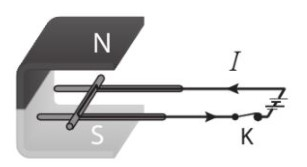
\includegraphics[width=0.3\linewidth]{figs/VN12-Y24-PH-SYL-018P-8}
	\end{center}
	\begin{enumerate}[label=\alph*)]
		\item Thanh kim loại sẽ lăn theo hướng nào khi đóng công tắc K?
		\item Nêu cách làm cho thanh kim loại lăn theo hướng ngược lại.
	\end{enumerate}
	\loigiai{
		\begin{enumerate}[label=\alph*)]
			\item Thanh kim loại dẫn điện sẽ lăn về bên phải.
			\item Đảo ngược chiều dòng điện hoặc đổi chiều của từ trường.
		\end{enumerate}	
	}
\end{ex}

% ===================================================================
\begin{ex}
	Xác định hướng của lực từ tác dụng lên các đoạn dây dẫn có dòng điện chạy qua, được đặt trong từ trường đều như các hình dưới đây:
	\begin{center}
		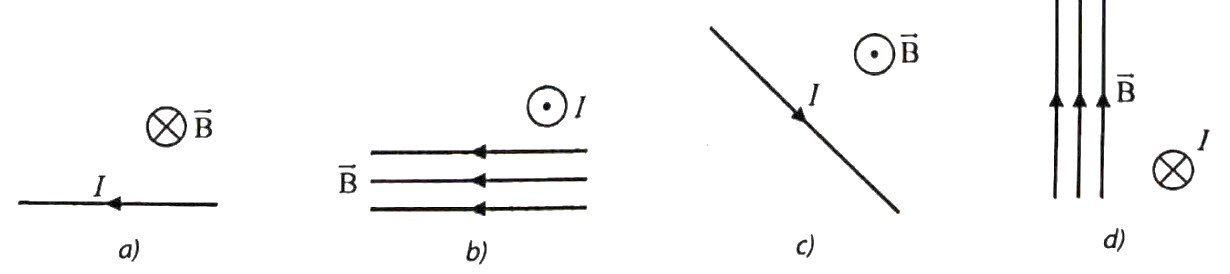
\includegraphics[width=0.8\linewidth]{figs/VN12-Y24-PH-SYL-018P-3}
	\end{center}
	\loigiai{
		\begin{center}
			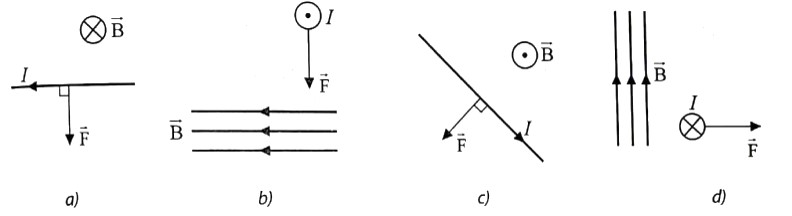
\includegraphics[width=0.8\linewidth]{figs/VN12-Y24-PH-SYL-018P-4}
		\end{center}	
	}
\end{ex}
% ======================================================================
\begin{ex}
	Xác định phương và chiều lực từ tác dụng lên các cạnh của khung. Biết chiều của vector cảm ứng từ $\vec{B}$ và chiều dòng điện được cho như mỗi hình vẽ.
	\begin{center}
		\begin{tabular}{cc}
			\begin{tikzpicture}
				\coordinate (A) at(0,0);
				\coordinate (B) at(0,-3);
				\coordinate (C) at(4,-3);
				\coordinate (D) at(0.5,0);
				\draw[decoration={markings, mark=at position 0.5 with{\arrow{stealth}}}, postaction={decorate}, line width=1.5pt](A)--(B)--(C)--(D);
				\foreach \y in {-0.5,-1.5,-2.5}{
					\draw[-latex, blue, line width=1.5pt] (-1,\y) --(4.5,\y);	
					\node[blue] at(4.5,0) {$\vec{B}$};
				}
				\node[left] at(A) {A};
				\node[left] at(B) {B};
				\node[right] at(C) {C};
				\node[above right] at(D) {D};
			\end{tikzpicture}
			&
			\begin{tikzpicture}
				\coordinate (A) at(0,0);
				\coordinate (B) at(0,-3);
				\coordinate (C) at(4,-3);
				\coordinate (D) at(4,0);
				\coordinate (E) at(0.5,0);
				\draw[decoration={markings, mark=at position 0.35 with{\arrow{stealth}}}, postaction={decorate}, line width=1.5pt](A)--(B)--(C)--(D)--(E);
				
				\node[left] at(A) {A};
				\node[left] at(B) {B};
				\node[right] at(C) {C};
				\node[right] at(D) {D};
				\node[above] at(E) {E};
				\node[blue] at(2,-1.5) {\LARGE $\odot$};
				\node[blue, right] at(2.2,-1.5) {$\vec{B}$};
			\end{tikzpicture}\\
			Hình a & Hình b
		\end{tabular}
	\end{center}
	\loigiai{
		\begin{center}
			\begin{tabular}{M{6cm}M{6cm}}
				\begin{tikzpicture}
					\coordinate (A) at(0,0);
					\coordinate (B) at(0,-3);
					\coordinate (C) at(4,-3);
					\coordinate (D) at(0.5,0);
					\draw[decoration={markings, mark=at position 0.5 with{\arrow{stealth}}}, postaction={decorate}, line width=1.5pt](A)--(B)--(C)--(D);
					\foreach \y in {-0.5,-1.5,-2.5}{
						\draw[-latex, blue, line width=1.5pt] (-1,\y) --(4.5,\y);	
						\node[blue] at(4.5,0) {$\vec{B}$};
					}
					\node[left] at(A) {A};
					\node[left] at(B) {B};
					\node[right] at(C) {C};
					\node[above right] at(D) {D};
					\node[red, fill=white, minimum size=0pt,inner sep=0pt, circle] at (0,-1.5) {\LARGE$\odot$};
					\node[red, below right] at (0.25,-1.5) {$\vec{F}_{\text{AB}}$};
					\node[red, fill=white, minimum size=0pt,inner sep=0pt, circle] at ($(D)!0.5!(C)$) {\LARGE$\otimes$};
					\node[red, below] at ($(D)!0.5!(C)+(0,-0.25)$) {$\vec{F}_{\text{CD}}$};
				\end{tikzpicture}
				&
				\begin{tikzpicture}
					\coordinate (A) at(0,0);
					\coordinate (B) at(0,-3);
					\coordinate (C) at(4,-3);
					\coordinate (D) at(4,0);
					\coordinate (E) at(0.5,0);
					\draw[decoration={markings, mark=at position 0.35 with{\arrow{stealth}}}, postaction={decorate}, line width=1.5pt](A)--(B)--(C)--(D)--(E);
					\draw[-latex, red, line width=1.5pt] ($(A)!0.5!(B)$)--+(-1,0);
					\draw[-latex, red, line width=1.5pt] ($(B)!0.5!(C)$)--+(0,-1);
					\draw[-latex, red, line width=1.5pt] ($(C)!0.5!(D)$)--+(1,0);
					\draw[-latex, red, line width=1.5pt] ($(D)!0.5!(E)$)--+(0,1);
					\node[left] at(A) {A};
					\node[left] at(B) {B};
					\node[right] at(C) {C};
					\node[right] at(D) {D};
					\node[above] at(E) {E};
					\node[blue] at(2,-1.5) {\LARGE $\odot$};
					\node[blue, right] at(2.2,-1.5) {$\vec{B}$};
					\node[red, above] at ($(A)!0.5!(B)+(-1,0)$) {$\vec{F}_{\text{AB}}$};
					\node[red, right] at ($(B)!0.5!(C)+(0,-1)$) {$\vec{F}_{\text{BC}}$};
					\node[red, above] at ($(C)!0.5!(D)+(1,0)$) {$\vec{F}_{\text{CD}}$};
					\node[red, right] at ($(D)!0.5!(E)+(0,1)$) {$\vec{F}_{\text{DE}}$};
				\end{tikzpicture}\\
				Hình a & Hình b
			\end{tabular}
		\end{center}	
	}
\end{ex}



% ===================================================================
\begin{ex}
	\immini{Động cơ điện là thiết bị có thể chuyển hoá năng lượng điện thành cơ năng (chuyển động quay của động cơ). Mô hình đơn giản của một động cơ điện gồm: một khung dây dẫn hình chữ nhật ABCD đang có dòng điện không đổi chạy qua. Khung dây được đặt vào trong từ trường đều có các đường sức từ thẳng đứng như hình bên. Tại thời điểm ban đầu, khung đang ở vị trí sao cho hai cạnh AB và CD đang song song với các đường sức từ. Vẽ các lực từ tác dụng lên các cạnh của khung dây. Các lực này có tác dụng làm cho khung dây chuyển động như thế nào?	}
	{
		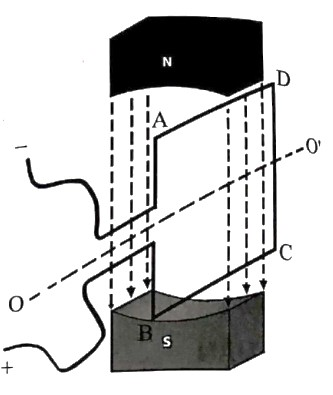
\includegraphics[width=0.45\linewidth]{figs/VN12-Y24-PH-SYL-018P-5}
	}
	\loigiai{
		Chỉ có lực từ tác dụng lên hai cạnh AD và BC của khung dây. Hai lực này tạo ra cặp ngẫu lực và có tác dụng tạo ra moment ngẫu lực làm quay khung dây.
		\begin{center}
			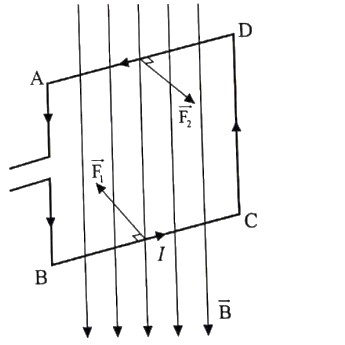
\includegraphics[width=0.4\linewidth]{figs/VN12-Y24-PH-SYL-018P-6}
		\end{center}	
	}
\end{ex}

% =================================================================
\begin{ex}
	Cho hai dây dẫn thẳng song song, dài vô hạn lần lượt có dòng điện $I_1$ và $I_2$ chạy qua như hình \ref{fig:17P-1}. Xét mặt phẳng $\left(Oxy\right)$ vuông góc với cả hai dòng điện, cắt các dòng điện tại A và B.
	\begin{center}
		\begin{tikzpicture}
			\coordinate (O) at (0,0);
			\coordinate (A) at ($(O)+(75:3)$);
			\coordinate (C) at (6,0);
			\coordinate (B) at ($(C)+(75:3)$);
			\fill[orange!50!white, opacity=0.6] (O)--(A)--(B)--(C)--(O);
			\draw[-latex, line width=1.5pt] (O)--+(75:4);
			\draw[-latex, line width=1.5pt] (O)--+(7,0);
			\draw[line width=1pt, dashed] (1,1.45)--(6,1.45);
			\draw[line width=1.5pt, blue,decoration={markings, mark=at position 0.625 with {\arrow{stealth}}},
			postaction={decorate}] 
			(1.5,1.45)--+(0,2.5);
			\draw[line width=1.5pt, blue, dashed] (1.5,1.45)--+(0,-1.45);
			\draw[line width=1.5pt, blue] (1.5,0)--+(0,-1);
			\draw[line width=1.5pt, blue,decoration={markings, mark=at position 0.625 with {\arrow{stealth}}},
			postaction={decorate}] 
			(3.5,1.45)--+(0,2.5);
			\draw[line width=1.5pt, blue, dashed] (3.5,1.45)--+(0,-1.45);
			\draw[line width=1.5pt, blue] (3.5,0)--+(0,-1);
			\filldraw (1.5,1.45) circle(2pt) node[above left] {A};
			\filldraw (3.5,1.45) circle(2pt) node[above left] {B};
			\filldraw (5,1.45) circle(2pt) node[above left] {C};
			\node[left] at (O) {O};
			\node[below] at (7,0) {$x$};
			\node[left] at ($(O)+(75:4)$) {$y$};
			\node[right] at (1.5,3) {$I_1$};
			\node[right] at (3.5,3) {$I_2$};
		\end{tikzpicture}
	\end{center}
	\captionof{figure}{}
	\label{fig:17P-1}
	\begin{enumerate}[label=\alph*)]
		\item Xác định phương, chiều của các vector cảm ứng từ do từng dòng điện gây ra tại C (A, B, C thẳng hàng).
		\item Nếu đặt một kim la bàn tại điểm C thì kim la bàn này sẽ định hướng như thế nào? Giải thích.
	\end{enumerate}
	\loigiai{\begin{enumerate}[label=\alph*)]
			\item Dựa vào quy tắc nắm tay phải, ta xác định được vector cảm ứng từ do hai dòng điện $I_1$ và $I_2$ gây ra tại điểm C đều nằm trong mặt phẳng $\left(Oxy\right)$, phương song song và cùng chiều với trục $Oy$.
			\item Hai vector cảm ứng từ do hai dòng điện $I_1$ và $I_2$ gây ra đều cùng hướng với nhau nên kim la bàn khi đặt tại C sẽ có cực Bắc hướng theo chiều dương trục $Oy$ còn cực Nam hướng ngược lại.
	\end{enumerate}}
\end{ex}
% ===================================================================
\begin{ex}
	Một dây dẫn có chiều dài $L=\SI{1.2}{\meter}$, được đặt trong từ trường đều có độ lớn $B=\SI{5E-2}{\tesla}$. Cường độ dòng điện chạy trong dây dẫn có giá trị $\SI{3}{\ampere}$. Hãy xác định độ lớn của lực từ tác dụng lên dây dẫn trong các trường hợp sau đây:
	\begin{enumerate}[label=\alph*)]
		\item Dây dẫn đặt vuông góc với các đường sức từ.
		\item Dây dẫn đặt song song với các đường sức từ.
		\item Dây dẫn hợp với các đường sức từ một góc $\SI{45}{\degree}$.
	\end{enumerate}	
	\loigiai{
		\begin{enumerate}[label=\alph*)]
			\item $F=ILB\sin\SI{90}{\degree}=\SI{0.18}{\newton}$.
			\item $F=ILB\sin\SI{0}{\degree}=\SI{0}{\newton}$.
			\item $F=ILB\sin\SI{45}{\degree}\approx\SI{0.13}{\newton}$.
		\end{enumerate}	
	}
\end{ex}
% ===================================================================
\begin{ex}
	Một đoạn dây dẫn thẳng dài $\SI{20}{\centi\meter}$ mang dòng điện có cường độ $\SI{50}{\milli\ampere}$ được đặt vào một vùng từ trường đều có cảm ứng từ $\SI{100}{\micro\tesla}$. Xác định góc hợp bởi đoạn dây và vector cảm ứng từ để lực từ tác dụng lên đoạn dây đạt độ lớn cực đại. Tính giá trị cực đại này.	
	\loigiai{
		Từ biểu thức tính độ lớn lực từ $F=B I L \sin \theta$, ta thấy lực từ đạt độ lớn cực đại khi: $\sin \theta=1 \Rightarrow \theta=\SI{90}{\degree}$. Khi đó, $F=B I L=100 \cdot 10^{-6} \cdot 50 \cdot 10^{-3} \cdot 0,2=\SI{E-6}{\newton}$.
		
	}
\end{ex}

% ===================================================================
\begin{ex}
	Một đoạn dây dẫn dài $\SI{5}{\centi\meter}$ đặt trong từ trường đều và vuông góc với vector cảm ứng từ. Dòng điện chạy qua dây có cường độ $\SI{0.75}{\ampere}$. Lực từ tác dụng lên đoạn dây đó là $\SI{3E-2}{\newton}$. Tính độ lớn cảm ứng từ.
	\loigiai{
		$$
		B=\frac{F}{IL\sin \theta}=\frac{3 \cdot 10^{-2}}{0,75 \cdot 0,05 \cdot \sin \SI{90}{\degree}}=\SI{0.8}{\tesla}.
		$$	
	}
\end{ex}
% ===================================================================
\begin{ex}
	Một đoạn dây dẫn dài $\SI{10}{\centi\meter}$ đặt trong từ trường đều, hợp với vector cảm ứng từ một góc $\SI{30}{\degree}$. Dòng điện có cường độ $\SI{2}{\ampere}$ chạy qua dây dẫn thì lực từ tác dụng lên đoạn dây có độ lớn là $\SI{4E-2}{\newton}$. Tính độ lớn của cảm ứng từ.
	\loigiai{
		Ta có: $\alpha=\SI{30}{\degree} \Rightarrow \sin \theta=\frac{1}{2}$. \\
		Cảm ứng từ của từ trường có độ lớn: $B=\dfrac{F}{IL\sin \theta}=\dfrac{4 \cdot 10^{-3}}{2 \cdot 0,1 \cdot 0,5}=\SI{0.04}{\tesla}$.	
	}
\end{ex}
% ===================================================================
\begin{ex}
	Một đoạn dây dẫn thẳng MN có chiều dài $\SI{6}{\centi\meter}$, có cường độ dòng điện $I=\SI{5}{\ampere}$ chạy qua đặt trong từ trường đều có cảm ứng từ $B=\SI{0.5}{\tesla}$. Lực từ tác dụng lên đoạn dây có độ lớn $F=\SI{7.5E-2}{\newton}$. Tính góc $\theta$ hợp bởi dây MN và vector cảm ứng từ.	
	\loigiai{
		Độ lớn của lực từ tác dụng lên đoạn dây dẫn có chiều dài $L$ mang dòng điện $I$ đặt trong từ trường cảm ứng từ $B$ là: $F=ILB \sin\theta \Rightarrow \sin\theta=0,5 \Rightarrow \theta=\SI{30}{\degree}.$	
	}
\end{ex}
% ===================================================================
\begin{ex}
	Một đoạn dây dài $L$ đặt trong từ trường đều có cảm ứng từ $B=\SI{0.5}{\tesla}$ hợp với đường cảm ứng từ một góc $\SI{30}{\degree}$. Dòng điện qua dây có cường độ $\SI{0.5}{\ampere}$, thì lực từ tác dụng lên đoạn dây là $\SI{4E-2}{\newton}$. Tính chiều dài đoạn dây dẫn.	
	\loigiai{
		Chiều dài đoạn dây dẫn:
		$$
		L=\frac{F}{IB \sin \theta}=\frac{4 \cdot 10^{-2}}{0,5 \cdot 0,5 \cdot \sin \SI{30}{\degree}}=\SI{0.32}{\meter}=\SI{32}{\centi\meter}.
		$$
		
	}
\end{ex}
% ===================================================================
\begin{ex}
	Một đoạn dây dẫn dài $L=\SI{0.5}{\meter}$ đặt trong từ trường đều sao cho dây dẫn hợp với vector cảm ứng từ một góc $\SI{45}{\degree}$. Biết cảm ứng từ $B=\SI{0.2}{\tesla}$ và dây dẫn chịu lực từ $F=\SI{4E-2}{\newton}$. Tính cường độ dòng điện chạy qua dây dẫn.
	\loigiai{
		$$
		I=\frac{F}{BL \sin \theta}=\frac{4 \cdot 10^{-2}}{0,2 \cdot 0,5 \cdot \sin \SI{45}{\degree}}=\xsi{0,4\sqrt{2}}{\ampere}.
		$$
		
	}
\end{ex}
% ===================================================================
\begin{ex}
	Một đường dây tải điện thẳng dài $\SI{42}{\meter}$ có dòng điện với cường độ $\SI{150}{\ampere}$ chạy qua theo hướng về phía Bắc. Từ trường Trái Đất tại vị trí này có độ lớn khoảng $\SI{0.5E-4}{\tesla}$, có hướng lệch một góc $\theta=\SI{50}{\degree}$ so với dòng điện. Xác định lực từ tác dụng lên đường dây nói trên.
	\begin{center}
		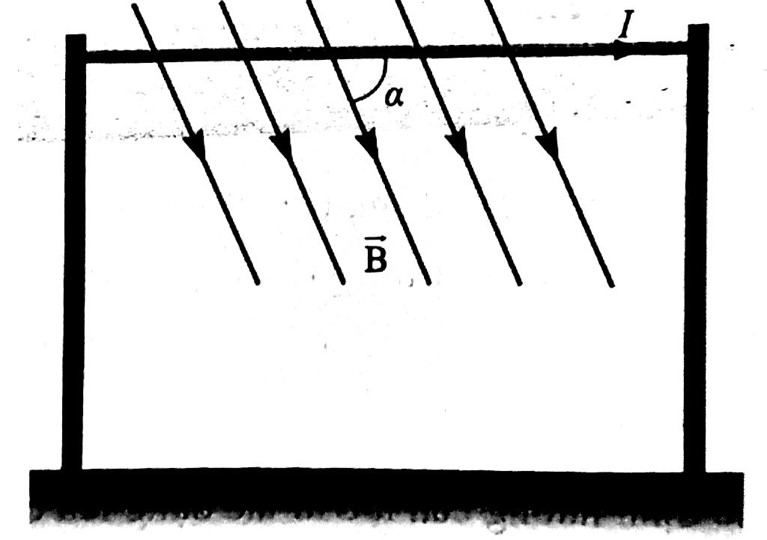
\includegraphics[width=0.4\linewidth]{figs/VN12-Y24-PH-SYL-018P-7}
	\end{center}
	\loigiai{
		Lực từ tác dụng lên đường dây có chiều hướng về phía Tây và có độ lớn là:
		$$F=B I L \sin \theta=0,5 \cdot 10^{-4} \cdot 150 \cdot 42 \cdot \sin \SI{50}{\degree} \approx \SI{0.24}{\newton}.$$
		
	}
\end{ex}
% ======================================================================
\begin{ex}
	Một dây dẫn có dòng điện $\SI{22.0}{\ampere}$ chạy từ Tây sang Đông. Giả sử tại vị trí này, từ trường Trái Đất nằm ngang và hướng từ Nam lên Bắc với độ lớn $\SI{0.5E-4}{\tesla}$.
	\begin{enumerate}[label=\alph*)]
		\item Tìm độ lớn và hướng của lực từ tác dụng lên một đoạn dây dài $\SI{36.0}{\meter}$.
		\item Tính lực hấp dẫn tác dụng lên đoạn dây có cùng chiều dài nếu nó được làm bằng đồng và có diện tích mặt cắt ngang là $\SI{2.50E-6}{\meter^2}$. Khối lượng riêng của đồng là $\SI{8.9E3}{\kilogram/\meter^3}$, lấy $g=\SI{9.80}{\meter/\second^2}$.
	\end{enumerate}
	\loigiai{
		\begin{enumerate}[label=\alph*)]
			\item $F_{\text{từ}}=ILB=\SI{3.96E-2}{\newton}$, hướng vuông góc với trang giấy, từ sau ra trước.
			\item $F_{\text{hấp dẫn}}=\rho gLS=\SI{7.85}{\newton}$.
			
		\end{enumerate}	
	}
\end{ex}
% ======================================================================
\begin{ex}
	Một dây dẫn thẳng, cứng, dài $\SI{20}{\centi\meter}$, có khối lượng $\SI{50}{\gram}$ được giữ nằm yên theo phương ngang trong một từ trường có độ lớn cảm ứng từ là $\SI{0.49}{\tesla}$ và có hướng nằm ngang, vuông góc với dây. Cường độ dòng điện chạy trong dây là bao nhiêu để khi dây được thả ra thì nó vẫn nằm yên? Lấy $g=\SI{9.8}{\meter/\second^2}$.
	
	\loigiai{
		$$F_{\text{từ}}	=P\Leftrightarrow ILB=mg\Rightarrow I=\dfrac{mg}{BL}=\SI{5.0}{\ampere}.$$
	}
\end{ex}

% ===================================================================
\begin{ex}
	Treo một đoạn dây dẫn có chiều dài $L=\SI{5}{\centi\meter}$, khối lượng $m=\SI{5}{\gram}$ bằng hai dây mảnh, nhẹ sao cho dây dẫn nằm ngang. Biết cảm ứng từ của từ trường hướng thẳng đứng xuống dưới, có độ lớn $B=\SI{0.5}{\tesla}$ và dòng điện chạy qua dây dẫn là $I=\SI{2}{\ampere}$. Lấy $g=\SI{10}{\meter/\second^2}$. Tính góc lệch của dây treo so với phương thẳng đứng.
	\loigiai{
		$$
		\tan \theta=\frac{F_t}{P}=\frac{0,5 \cdot 2 \cdot 0,05}{0,005 \cdot 10}=1 \Rightarrow \theta=\SI{45}{\degree}.
		$$
		
	}
\end{ex}
% ===================================================================
\begin{ex}
	Một đoạn dây dẫn thẳng MN có chiều dài $L=\SI{6}{\centi\meter}$, có dòng điện cường độ $I=\SI{5}{\ampere}$ chạy qua đặt trong từ trường đều có cảm ứng từ $B=\SI{0.5}{\tesla}$. Lực từ tác dụng lên đoạn dây có độ lớn $F=\SI{7.5E-2}{\newton}$. Tính góc $\theta$ hợp bởi dây MN và vector cảm ứng từ.
	\loigiai{
		Áp dụng công thức $F=ILB \sin \theta$ với $L=\SI{6E-2}{\meter}, I=\SI{5}{\ampere}, F=\SI{7.5E-2}{\newton}$ và $B=\SI{0.5}{\tesla}$, ta tính được $\theta=\SI{30}{\degree}$.
		
	}
\end{ex}
% ======================================================================
\begin{ex}
	Thanh MN dài $\ell=\SI{20}{\centi\meter}$ có khối lượng $\SI{5}{\gram}$ treo nằm ngang bằng hai sợi chỉ mảnh CM và DN. Thanh nằm trong từ trường đều có cảm ứng từ	 $B=\SI{0.3}{\tesla}$ nằm ngang vuông góc với thanh có chiều như hình vẽ. Mỗi sợi chỉ treo thanh có thể chịu được lực kéo tối đa là $\SI{0.04}{\newton}$. Dòng điện chạy qua thanh MN có chiều và cường độ lớn nhất là bao nhiêu thì sợi chỉ treo thanh chưa bị đứt. Lấy gia tốc trọng trường $g=\SI{9.8}{\meter/\second^2}$.
	\begin{center}
		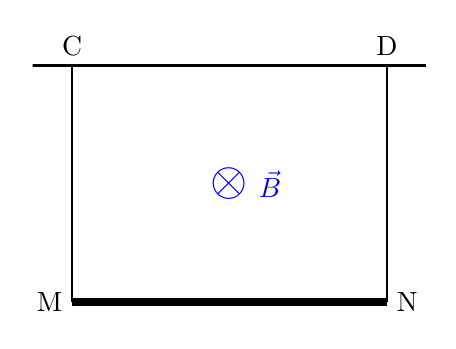
\begin{tikzpicture}
			\coordinate (C) at (0,0);
			\coordinate (D) at (4,0);
			\coordinate (M) at (0,-3);
			\coordinate (N) at (4,-3);
			\draw[line width=1pt] (C)--+(-0.5,0)--+(4.5,0);
			\draw[line width=1pt] (C)--(M);
			\draw[line width=1pt] (D)--(N);
			\draw[line width=3pt] (M)--(N);
			\node[blue] at (2,-1.5) {\LARGE$\otimes$};
			\node[blue, right] at (2.25,-1.5) {$\vec{B}$};
			\node[above] at (C) {C};
			\node[above] at (D) {D};
			\node[left] at (M) {M};
			\node[right] at (N) {N};
		\end{tikzpicture}
	\end{center}
	\loigiai{
		Khi cho dòng điện chạy qua dây dẫn đặt trong từ trường thì sẽ có lực từ tác dụng lên dây dẫn.
		\begin{itemize}
			\item Công thức tính lực từ: $F=IB \ell \sin \alpha$.
			\item Dây bị đứt khi lực từ hướng xuống.\\
			Để dây không đứt thì $P+F \leq 2 T \Rightarrow F \leq 2T-P$
			$$
			\begin{aligned}
				& \Rightarrow F_{\text{max}}=BI_{\text{max}} \ell \sin \SI{90}{\degree}=2T-mg \\
				& \Rightarrow I_{\text{max}}=\frac{2 T-mg}{B\ell} \\
				& \Rightarrow I_{\text{max}}=\frac{2 \cdot 0,04-0,005 \cdot 9,8}{0,3 \cdot 0,2}\approx \SI{0.52}{\ampere}.
			\end{aligned}
			$$
		\end{itemize}
		Xác định chiều của dòng điện bằng cách sử dụng quy tắc bàn tay trái. Để lực từ hướng xuống thì dòng điện phải có chiều từ N đến M.	
	}
\end{ex}



% ======================================================================
\begin{ex}
	Một dây dẫn được gập thành khung dây dạng tam giác vuông cân MNP với $\mathrm{MN}=\mathrm{NP}=\SI{10}{\centi\meter}$. Đặt khung dây vào từ trường $B=\SI{E-2}{\tesla}$ có chiều như hình vẽ. Cho dòng điện có cường độ $I=\SI{10}{\ampere}$ vào khung theo chiều MNPM. Lực từ tác dụng vào các cạnh của khung dây là bao nhiêu?
	\begin{center}
		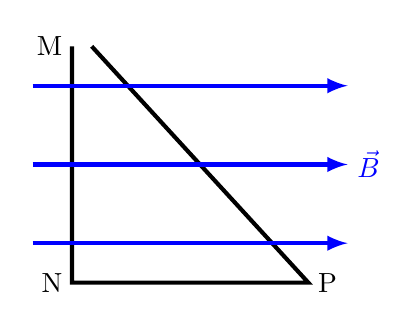
\begin{tikzpicture}
			\coordinate (M) at(0,0);
			\coordinate (N) at(0,-3);
			\coordinate (P) at(3,-3);
			\coordinate (Q) at(0.25,0);
			\draw[line width=1.5pt] (M)--(N)--(P)--(Q);
			\foreach \y in {-0.5,-1.5,-2.5}{
				\draw[-latex, blue, line width=1.5pt] (-0.5,\y)--(3.5,\y);	
			}
			\node[left] at(M) {M};
			\node[left] at(N) {N};
			\node[right] at(P) {P};
			\node[blue,right] at (3.5,-1.5) {$\vec{B}$};
		\end{tikzpicture}
	\end{center}
	\loigiai{
		\begin{itemize}
			\item Vì MN vuông với $\vec{B}$ nên:
			$$F_\mathrm{MN}=BIL\sin\SI{90}{\degree}=\SI{E-2}{\newton}.$$
			\item Vì NP song song với $\vec{B}$ nên:
			$$
			F_\mathrm{NP}=B I L \sin \SI{0}{\degree}=0
			$$
			\item  Từ hình ta thấy $\overrightarrow{PM}$ tạo với $\vec{B}$ một góc:
			$$
			\alpha=180-45=\SI{135}{\degree}
			$$
			Do đó lực tác dụng lên đoạn PM là:
			$$
			F_\mathrm{PM}=B I L \sin \SI{135}{\degree}=\SI{E-2}{\newton}.
			$$
		\end{itemize}	
	}
\end{ex}
% ======================================================================
\begin{ex}
	Trong giờ thực hành đo độ lớn cảm ứng từ bằng "cân dòng điện" với bố trí thí nghiệm được thể hiện như trong hình 11.1 (dụng cụ thí nghiệm và các bước tiến hành thí nghiệm lần lượt được trình bày ở Bài 10 và Bài 11 trong SGK), một bạn học sinh đã thu được bảng số liệu như bảng dưới đây. Hãy xử lí số liệu thu được để đưa ra kết quả độ lớn cảm ứng từ trong thí nghiệm này.
	\begin{center}
		\begin{tabular}{|M{2cm}|M{2cm}|M{2cm}|M{2cm}|M{4cm}|M{3.5cm}|}
			\hline
			\multicolumn{6}{|M{17cm}|}{$\theta=\SI{90}{\degree}$; $L=\SI{0.04}{\meter}$; $N=\SI{200}{\text{vòng}}$}\\
			\hline
			\thead{Lần đo} & $\xsi{I}{\left(\ampere\right)}$ & $\xsi{F_1}{\left(\newton\right)}$ & $\xsi{F_2}{\left(\newton\right)}$ & $F=\xsi{F_2-F_1}{\left(\newton\right)}$ & $B=\xsi{\frac{F}{NIL}}{\left(\tesla\right)}$\\
			\hline
			1 & 0,4 & 0,210 & 0,320 &&\\
			\hline
			2 & 0,8 & 0,220 & 0,440 & &\\
			\hline
			3 & 1,0 & 0,200 & 0,480 & &\\
			\hline
			\multicolumn{5}{|M{12cm}|}{\thead{Trung bình}} &$\overline{B}=$\\
			\hline
			
		\end{tabular}
	\end{center}	
	\loigiai{
		\begin{center}
			\begin{tabular}{|M{2cm}|M{2cm}|M{2cm}|M{2cm}|M{4cm}|M{3.5cm}|}
				\hline
				\multicolumn{6}{|M{17cm}|}{$\theta=\SI{90}{\degree}$; $L=\SI{0.04}{\meter}$; $N=\SI{200}{\text{vòng}}$}\\
				\hline
				\thead{Lần đo} & $\xsi{I}{\left(\ampere\right)}$ & $\xsi{F_1}{\left(\newton\right)}$ & $\xsi{F_2}{\left(\newton\right)}$ & $F=\xsi{F_2-F_1}{\left(\newton\right)}$ & $B=\xsi{\frac{F}{NIL}}{\left(\tesla\right)}$\\
				\hline
				1 & 0,4 & 0,210 & 0,320 &0,110&0,034\\
				\hline
				2 & 0,8 & 0,220 & 0,440 &0,220 &0,034\\
				\hline
				3 & 1,0 & 0,200 & 0,480 &0,280 &0,035\\
				\hline
				\multicolumn{5}{|M{12cm}|}{\thead{Trung bình}} &$\overline{B}=0,0343$\\
				\hline
				
			\end{tabular}
		\end{center}		
	}
\end{ex}

% ======================================================================
\begin{ex}
	Sơ đồ bố trí thí nghiệm dưới đây được sử dụng để xác định độ lớn cảm ứng từ $B$ giữa các cực của nam châm.\\
	Nam châm được đặt trên cân. Dây dẫn mang dòng điện được đặt cố định nằm ngang và vuông góc với từ trường giữa các cực của nam châm. Lấy gia tốc rơi tự do $g=\SI{9.8}{\meter/\second^2}$.
	\begin{center}
		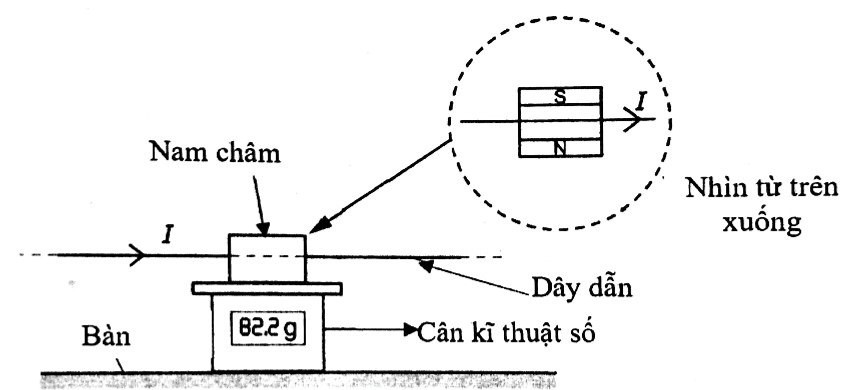
\includegraphics[width=0.6\linewidth]{figs/VN12-Y24-PH-SYL-018P-9}
	\end{center}
	Số liệu thu thập được như sau:
	\begin{itemize}
		\item Chiều dài của dây trong từ trường đều của nam châm: $\ell=\xsi{6,0\pm 0,2}{\centi\meter}$;
		\item Số chỉ của cân khi không có dòng điện trong dây dẫn: $\SI{80,0}{\gram}$;
		\item Số chỉ của cân khi có dòng điện trong dây: $\SI{82.2}{\gram}$;
		\item Dòng điện trong dây: $I=\xsi{5,0\pm0,1}{\ampere}$.
	\end{itemize}
	Viết kết quả đo giá trị của $B$. Bỏ qua sai số của cân.
	\loigiai{
		Dây dẫn đặt trong từ trường nam châm nên chịu tác dụng lực từ $F$.\\
		Lực $F$ hướng xuống tác dụng lên cân giống như một trọng lực $\mathrm{P}=\mathrm{mg}$.
		Với $m$ là chênh lệch số chỉ đọc ở cân khi có và không có dòng điện trong dây:
		$$
		\begin{aligned}
			& m=82,2-80,0=\SI{2.2}{\gram} \\
			& F=m g=2,2 \cdot 10^{-3} \cdot 9,8=\SI{0.0216}{\newton} \\
			& B=\frac{F}{I \ell \sin \alpha}=\frac{0,0216}{5,0.0,06 \cdot \sin \SI{90}{\degree}}\approx\SI{0.072}{\tesla}
		\end{aligned}
		$$
		
		Bỏ qua sai số của $F$ thì:
		$$
		\frac{\Delta B}{B}=\frac{\Delta I}{I}+\frac{\Delta \ell}{\ell} \Leftrightarrow \frac{\Delta B}{0,072}=\frac{0,1}{5}+\frac{0,2}{6} \Rightarrow \Delta B\approx0,004 T
		$$
		
		Kết quả đo: $B=\overline{B} \pm \Delta B=0,072 \pm \SI{0.004}{\tesla}$	
	}
\end{ex}